% =====================================================================
%  MSc Dissertation — master file
%  Lattice-based adaptor signatures on CRYSTALS-Dilithium primitives
%  Class: muthesis (University of Manchester, Dept. of Computer Science)
%  Build:  make            (see Makefile) — pdflatex + bibtex + pdflatex x2
% =====================================================================
%
% Structure follows research_writing_guide.md (rubric-aligned):
%   Abstract / Contents / 1 Introduction (incl. brief lit review) /
%   2 Methodology / 3 Results and discussion / 4 Evaluation and Reflection /
%   5 Conclusion & future work / References.
% NOTE (deliberate): there is NO separate Background chapter — the literature
% review folds into the Introduction, as the assessment rubric requires.
%
% Use `singlespace` ONLY for drafts; remove before submission.
% The `wordcount` option prints the count from word.count under the table of
% contents (muthesis.cls: "A word count now (Sep 17) seems to be required").
% Regenerate word.count first:
%   texcount -1 -sum -relaxed -inc report.tex > word.count
\documentclass[12pt,MSc,wordcount,anon]{muthesis}

% Silences "PDF inclusion: found PDF version <1.7>, but at most version <1.5> allowed",
% raised by figures/fig_criterion_presign.pdf.  Raising the TARGET is deliberate rather
% than re-saving that figure at 1.5: it is the exempt Criterion plot whose text is
% outlined (the type gate cannot judge it), so it must not be rewritten.  PDF 1.7 is
% ISO 32000-1 and universally readable, and pdfTeX is the engine here, so the primitive
% applies; it must stay in the preamble, before any page is shipped out.
\pdfminorversion=7

% ---- packages (keep minimal; add as needed) ----
\usepackage[T1]{fontenc}
\usepackage[utf8]{inputenc}
\usepackage{lmodern}
\usepackage{microtype}
\usepackage{amsmath,amssymb}
\usepackage{booktabs}        % \toprule \midrule \bottomrule
\usepackage{array}           % ragged-right fixed-width columns (see \newcolumntype L below)
\newcolumntype{L}[1]{>{\raggedright\arraybackslash}p{#1}}  % left-aligned wrapping column
\usepackage{longtable}       % page-breaking tables (tab:challenges is taller than a page)
\usepackage{float}           % [H] for appendix reference tables that should not float
\usepackage{graphicx}
\usepackage{xcolor}
\usepackage{tikz}
\usetikzlibrary{arrows.meta,positioning,calc}
\usepackage{listings}        % code snippets (appendix only)
\usepackage[hidelinks]{hyperref}
\usepackage{cleveref}        % \cref / \Cref — load AFTER hyperref

% number figures/tables/equations by section (rubric requirement)
\numberwithin{equation}{chapter}
\numberwithin{figure}{chapter}
\numberwithin{table}{chapter}

% a lightweight TODO marker so gaps are visible while drafting
\newcommand{\TODO}[1]{\textcolor{red}{\textbf{[TODO: #1]}}}

% In-text citations are IEEE-style throughout: a bracketed number, never used as a word
% of the sentence. Where the authors are named the form is "Esgin et al.\ \cite{...}",
% with the number immediately after the name; otherwise the number attaches to a noun or
% a preposition ("Figure~1 in \cite{...}", "assumed in \cite{...}"). A \textcite shim
% used to live here for name+cite rendering; it had one call site and rendered
% identically to \cite, so both were removed rather than kept as a second spelling.

% consistent maths shorthands used across chapters
\newcommand{\Rq}{R_q}
\newcommand{\vecz}{\mathbf{z}}
\newcommand{\inftynorm}[1]{\lVert #1 \rVert_\infty}

% Measured benchmark numbers -- AUTO-GENERATED from the latest evidence run by
% scripts/gen_report_data.py (via scripts/sync_report.sh). Chapters must cite
% measured values ONLY through these macros (and the generated/tab_*.tex
% tables), never as hand-typed literals, so the report always reflects the
% latest run.
% AUTO-GENERATED by scripts/gen_report_data.py -- DO NOT EDIT.
% Regenerate with scripts/sync_report.sh (runs after every benchmark suite).
% Evidence run: 20260828_144608  (git c41bbb5)
% Source: evidence/latest/tables/*.csv
% Source: evidence/latest/logs/*.log
% Source: rust/fips204-las/*.log
\newcommand{\benchRunId}{20260828\_144608}
\newcommand{\benchGitShort}{c41bbb5}
\newcommand{\benchReps}{5}
\newcommand{\benchItersSign}{500}
\newcommand{\benchItersVerify}{1000}
\newcommand{\tamperFlips}{6736}
\newcommand{\ovPreSign}{2.2}
\newcommand{\ovPreVerify}{5.1}
\newcommand{\ovAdapt}{7.4}
\newcommand{\ovMaxAll}{8.2}
\newcommand{\packedOvPreSign}{15.8}
\newcommand{\packedOvPreVerify}{37.9}
\newcommand{\packedOvAdapt}{84.4}
\newcommand{\extMean}{35.9}
\newcommand{\setupMin}{22}
\newcommand{\setupMax}{79}
\newcommand{\rejAttBase}{2.696}
\newcommand{\rejAttLas}{2.804}
\newcommand{\rejAccBase}{37.1}
\newcommand{\rejAccLas}{35.7}
\newcommand{\sigBytesTwo}{4640}
\newcommand{\pkBytesTwo}{2944}
\newcommand{\sigBytesTarget}{6736}
\newcommand{\pkBytesTarget}{4416}
\newcommand{\stmtBytesTarget}{4416}
\newcommand{\witBytesTarget}{704}
\newcommand{\zPctTwo}{99.3}
\newcommand{\zPctTarget}{99.3}
\newcommand{\zPctFive}{99.3}
\newcommand{\clReps}{10}
\newcommand{\clIters}{1000}
\newcommand{\clSigBytes}{64}
\newcommand{\clPkBytes}{33}
\newcommand{\clPreSigBytes}{162}
\newcommand{\clRatioSig}{72}
\newcommand{\clRatioPk}{89}
\newcommand{\clRatioTimeMax}{300}
\newcommand{\clRatioTimeMaxOp}{Adapt}
\newcommand{\clOvPreSignX}{4.5}
\newcommand{\clOvPreVerifyX}{4.0}
\newcommand{\clAdaptUs}{1.3}
\newcommand{\lasAdaptPackedUs}{399}
\newcommand{\adaptPreVerifyPct}{63}
\newcommand{\clAdaptMatchedUs}{102}
\newcommand{\clRatioAdaptMatched}{4}
\newcommand{\adaptCodecKB}{15.3}
\newcommand{\mldsaIters}{200}
\newcommand{\mldsaContract}{13/13}
\newcommand{\mldsaNaiveP}{0}
\newcommand{\mldsaRepairedP}{200}
\newcommand{\mldsaOvPreSign}{2.8}
\newcommand{\mldsaOvPreSignSimp}{2.2}
\newcommand{\mldsaAttempts}{5.2172}
\newcommand{\mldsaAttemptsSimp}{2.7136}
\newcommand{\mldsaSigBytes}{3309}
\newcommand{\mldsaSigBytesSimp}{6736}
\newcommand{\mldsaSigRatio}{0.49}
\newcommand{\mldsaStmtBytes}{4416}
\newcommand{\mldsaStmtRatio}{1.00}
\newcommand{\mldsaPayloadRatio}{0.69}
\newcommand{\gasClassical}{75\,763}
\newcommand{\gasLasFloor}{290\,640}
\newcommand{\gasLasVerified}{56\,647\,414}
\newcommand{\gasLasVerifiedM}{56.6}
\newcommand{\gasRatioFloor}{3.8}
\newcommand{\gasRatioVerified}{748}
\newcommand{\gasCapOver}{3.4}
\newcommand{\gasLasOpt}{16\,438\,275}
\newcommand{\gasRatioOpt}{217}
\newcommand{\piKnowledgeError}{127}
\newcommand{\piProofBytes}{32\,046}
\newcommand{\gasOptReceipt}{16\,413\,275}
\newcommand{\gasOptCapPct}{97.8}
\newcommand{\gasOptHeadroom}{363\,941}
\newcommand{\gasOptCalldata}{50\,148}
\newcommand{\gasDTwoTotal}{10\,956\,784}
\newcommand{\gasDTwoCapPct}{65}
\newcommand{\gasDTwoHeadroom}{5\,820\,432}
\newcommand{\rustOvPreSign}{3.5}
\newcommand{\rustOvPreVerify}{-0.7}
\newcommand{\rustOvAdapt}{4.2}
\newcommand{\rustPackedOvPreSign}{1.4}
\newcommand{\rustPackedOvPreVerify}{17.5}
\newcommand{\rustPackedOvAdapt}{30.9}
\newcommand{\rustAttBase}{2.70}
\newcommand{\rustAttLas}{2.77}
\newcommand{\rustAccBase}{37.0}
\newcommand{\rustAccLas}{36.1}
\newcommand{\rustCMaxDev}{196}
\newcommand{\rustCMaxDevOp}{KeyGen}
\newcommand{\critSamples}{300}
\newcommand{\katDigestHead}{b4a10ffb}
\newcommand{\katDigestTail}{03be}


% Stage-2 (UTXO atomic swap) measurements -- AUTO-GENERATED from the captured
% bench_swap log by scripts/gen_stage2_data.py. Same rule as above: chapters
% cite these macros, never hand-typed literals.
% AUTO-GENERATED by scripts/gen_stage2_data.py -- DO NOT EDIT.
% Regenerate from a captured bench_swap log; never hand-type a measurement.
% Stage-2 evidence run: 20260730_162109  (git 4aef1f7)

\newcommand{\stageTwoRunId}{20260730\_162109}
\newcommand{\stageTwoGit}{4aef1f7}
\newcommand{\stageTwoCpu}{AMD Ryzen 7 7745HX with Radeon Graphics}
\newcommand{\stageTwoHost}{Linux 6.18.33.2-microsoft-standard-WSL2 x86\_64}
\newcommand{\stageTwoRustc}{rustc 1.96.0 (ac68faa20 2026-05-25)}
\newcommand{\stageTwoRuns}{10}
\newcommand{\stageTwoSeed}{6c61732d73776170\ldots}
\newcommand{\stageTwoLasSetup}{956.572µs}

\newcommand{\cfgOneSigName}{ECDSA adaptor signature (libsecp256k1-zkp)}
\newcommand{\cfgOneSigParams}{secp256k1, 256-bit group, $\sim$128-bit classical security (no post-quantum security)}
\newcommand{\cfgOnePiName}{none required}
\newcommand{\cfgOneBinding}{e9bd349c4e73a797}
\newcommand{\cfgOneFullyPQ}{no}
\newcommand{\cfgOneKeyMatMean}{58.4}
\newcommand{\cfgOneKeyMatSD}{9.7}
\newcommand{\cfgOnePreSignAMean}{114.9}
\newcommand{\cfgOnePreSignASD}{18.4}
\newcommand{\cfgOnePreVerifyMean}{147.6}
\newcommand{\cfgOnePreVerifySD}{35.1}
\newcommand{\cfgOnePreSignBMean}{107.1}
\newcommand{\cfgOnePreSignBSD}{14.5}
\newcommand{\cfgOneAdaptAMean}{138.4}
\newcommand{\cfgOneAdaptASD}{16.4}
\newcommand{\cfgOneSettleBMean}{51.9}
\newcommand{\cfgOneSettleBSD}{16.7}
\newcommand{\cfgOneExtMean}{25.3}
\newcommand{\cfgOneExtSD}{4.5}
\newcommand{\cfgOneAdaptBMean}{132.7}
\newcommand{\cfgOneAdaptBSD}{19.3}
\newcommand{\cfgOneSettleAMean}{43.4}
\newcommand{\cfgOneSettleASD}{7.8}
\newcommand{\cfgOneTotalMean}{819.7}
\newcommand{\cfgOneTotalSD}{93.1}
\newcommand{\cfgOneMsgY}{33}
\newcommand{\cfgOneMsgPreSigA}{162}
\newcommand{\cfgOneMsgTxA}{114}
\newcommand{\cfgOneMsgPreSigB}{162}
\newcommand{\cfgOneMsgTxB}{114}
\newcommand{\cfgOneMsgChainB}{178}
\newcommand{\cfgOneMsgChainA}{178}
\newcommand{\cfgOneBytesOffChain}{585}
\newcommand{\cfgOneBytesOnChain}{356}
\newcommand{\cfgOneBytesTotal}{941}
\newcommand{\cfgOneBytesPk}{33}
\newcommand{\cfgOneBytesSk}{32}
\newcommand{\cfgOneBytesStatement}{33}
\newcommand{\cfgOneBytesWitness}{32}
\newcommand{\cfgOneBytesSig}{64}
\newcommand{\cfgOneBytesPreSig}{162}
\newcommand{\cfgOneBytesPreSigOverhead}{98}

\newcommand{\cfgTwoSigName}{LAS (simplified Dilithium-III)}
\newcommand{\cfgTwoSigParams}{n=6, ell=5, n+ell=11, d=256, kappa=49, gamma=137984, q=8380417}
\newcommand{\cfgTwoPiName}{Groth16 over BN254 (pairing-based zk-SNARK)}
\newcommand{\cfgTwoBinding}{33c1947f2ba13f98}
\newcommand{\cfgTwoFullyPQ}{no}
\newcommand{\cfgTwoSetupKind}{trusted, per circuit (soundness requires the setup secret to be destroyed)}
\newcommand{\cfgTwoSetupTime}{1.225142318s}
\newcommand{\cfgTwoKeyMatMean}{540.7}
\newcommand{\cfgTwoKeyMatSD}{75.3}
\newcommand{\cfgTwoProveMean}{645621.6}
\newcommand{\cfgTwoProveSD}{57578.0}
\newcommand{\cfgTwoPreSignAMean}{1065.3}
\newcommand{\cfgTwoPreSignASD}{480.7}
\newcommand{\cfgTwoProofVerifyMean}{13718.1}
\newcommand{\cfgTwoProofVerifySD}{740.4}
\newcommand{\cfgTwoPreVerifyMean}{364.9}
\newcommand{\cfgTwoPreVerifySD}{32.3}
\newcommand{\cfgTwoPreSignBMean}{1070.1}
\newcommand{\cfgTwoPreSignBSD}{843.7}
\newcommand{\cfgTwoAdaptAMean}{392.5}
\newcommand{\cfgTwoAdaptASD}{37.7}
\newcommand{\cfgTwoSettleBMean}{253.0}
\newcommand{\cfgTwoSettleBSD}{26.0}
\newcommand{\cfgTwoExtMean}{185.2}
\newcommand{\cfgTwoExtSD}{10.2}
\newcommand{\cfgTwoAdaptBMean}{353.8}
\newcommand{\cfgTwoAdaptBSD}{37.5}
\newcommand{\cfgTwoSettleAMean}{243.0}
\newcommand{\cfgTwoSettleASD}{29.5}
\newcommand{\cfgTwoTotalMean}{663808.3}
\newcommand{\cfgTwoTotalSD}{57331.6}
\newcommand{\cfgTwoProofShare}{659339.7}
\newcommand{\cfgTwoProofPct}{99.3}
\newcommand{\cfgTwoMsgY}{4416}
\newcommand{\cfgTwoMsgPi}{128}
\newcommand{\cfgTwoMsgPreSigA}{6736}
\newcommand{\cfgTwoMsgTxA}{4497}
\newcommand{\cfgTwoMsgPreSigB}{6736}
\newcommand{\cfgTwoMsgTxB}{4497}
\newcommand{\cfgTwoMsgChainB}{11233}
\newcommand{\cfgTwoMsgChainA}{11233}
\newcommand{\cfgTwoBytesOffChain}{27010}
\newcommand{\cfgTwoBytesOnChain}{22466}
\newcommand{\cfgTwoBytesTotal}{49476}
\newcommand{\cfgTwoBytesPk}{4416}
\newcommand{\cfgTwoBytesSk}{704}
\newcommand{\cfgTwoBytesStatement}{4416}
\newcommand{\cfgTwoBytesWitness}{704}
\newcommand{\cfgTwoBytesSig}{6736}
\newcommand{\cfgTwoBytesPreSig}{6736}
\newcommand{\cfgTwoBytesPreSigOverhead}{0}
\newcommand{\cfgTwoRejMeasured}{2.8510}
\newcommand{\cfgTwoRejExpected}{2.77483}
\newcommand{\cfgTwoRejTol}{0.2481}
\newcommand{\cfgTwoRejCalls}{2000}

\newcommand{\cfgThreeSigName}{LAS (simplified Dilithium-III)}
\newcommand{\cfgThreeSigParams}{n=6, ell=5, n+ell=11, d=256, kappa=49, gamma=137984, q=8380417}
\newcommand{\cfgThreePiName}{LaZer (LNP22 linear relation with norms)}
\newcommand{\cfgThreeBinding}{33c1947f2ba13f98}
\newcommand{\cfgThreeFullyPQ}{yes}
\newcommand{\cfgThreeSetupKind}{transparent (public-coin; no trusted party)}
\newcommand{\cfgThreeSetupTime}{0ns}
\newcommand{\cfgThreeKeyMatMean}{503.2}
\newcommand{\cfgThreeKeyMatSD}{18.2}
\newcommand{\cfgThreeProveMean}{216080.6}
\newcommand{\cfgThreeProveSD}{81290.2}
\newcommand{\cfgThreePreSignAMean}{1065.7}
\newcommand{\cfgThreePreSignASD}{441.9}
\newcommand{\cfgThreeProofVerifyMean}{90720.8}
\newcommand{\cfgThreeProofVerifySD}{7577.8}
\newcommand{\cfgThreePreVerifyMean}{380.2}
\newcommand{\cfgThreePreVerifySD}{26.7}
\newcommand{\cfgThreePreSignBMean}{966.7}
\newcommand{\cfgThreePreSignBSD}{811.2}
\newcommand{\cfgThreeAdaptAMean}{380.5}
\newcommand{\cfgThreeAdaptASD}{49.7}
\newcommand{\cfgThreeSettleBMean}{239.9}
\newcommand{\cfgThreeSettleBSD}{15.4}
\newcommand{\cfgThreeExtMean}{183.6}
\newcommand{\cfgThreeExtSD}{8.0}
\newcommand{\cfgThreeAdaptBMean}{340.9}
\newcommand{\cfgThreeAdaptBSD}{13.6}
\newcommand{\cfgThreeSettleAMean}{234.9}
\newcommand{\cfgThreeSettleASD}{6.5}
\newcommand{\cfgThreeTotalMean}{311097.1}
\newcommand{\cfgThreeTotalSD}{83471.0}
\newcommand{\cfgThreeProofShare}{306801.4}
\newcommand{\cfgThreeProofPct}{98.6}
\newcommand{\cfgThreeMsgY}{4416}
\newcommand{\cfgThreeMsgPi}{30711--30760}
\newcommand{\cfgThreeMsgPreSigA}{6736}
\newcommand{\cfgThreeMsgTxA}{4497}
\newcommand{\cfgThreeMsgPreSigB}{6736}
\newcommand{\cfgThreeMsgTxB}{4497}
\newcommand{\cfgThreeMsgChainB}{11233}
\newcommand{\cfgThreeMsgChainA}{11233}
\newcommand{\cfgThreeBytesOffChain}{57593--57642}
\newcommand{\cfgThreeBytesOnChain}{22466}
\newcommand{\cfgThreeBytesTotal}{80059--80108}
\newcommand{\cfgThreeBytesPk}{4416}
\newcommand{\cfgThreeBytesSk}{704}
\newcommand{\cfgThreeBytesStatement}{4416}
\newcommand{\cfgThreeBytesWitness}{704}
\newcommand{\cfgThreeBytesSig}{6736}
\newcommand{\cfgThreeBytesPreSig}{6736}
\newcommand{\cfgThreeBytesPreSigOverhead}{0}
\newcommand{\cfgThreeRejMeasured}{2.8510}
\newcommand{\cfgThreeRejExpected}{2.77483}
\newcommand{\cfgThreeRejTol}{0.2481}
\newcommand{\cfgThreeRejCalls}{2000}

\newcommand{\cmpTimeFrom}{663808.3}
\newcommand{\cmpTimeTo}{311097.1}
\newcommand{\cmpTimePct}{-53.1}
\newcommand{\cmpBytesFrom}{49476}
\newcommand{\cmpBytesTo}{80059--80108}
\newcommand{\cmpBytesPct}{+61.9}
\newcommand{\cmpProofFrom}{128}
\newcommand{\cmpProofTo}{30711--30760}
\newcommand{\cmpTimePctAbs}{53.1}
\newcommand{\cmpBytesPctAbs}{61.9}

% derived (computed by the generator, not measured directly)
\newcommand{\cfgOneNonProofUs}{819.7}
\newcommand{\cfgTwoNonProofUs}{4468.6}
\newcommand{\cfgThreeNonProofUs}{4295.7}
\newcommand{\stageTwoCryptoRatio}{5.5}
\newcommand{\stageTwoBytesRatioTwo}{52.6}
\newcommand{\stageTwoBytesRatioThree}{85.1}
\newcommand{\stageTwoOnChainRatio}{63.1}
\newcommand{\stageTwoProofSizeRatio}{240}


% Bitcoin wire-format projection of the settled swap transaction -- AUTO-GENERATED
% by scripts/gen_bitcoin_tx_data.py from the same bench_swap log. Object sizes are
% measured; the field layout is BIP141/BIP144/BIP341; the arithmetic self-checks
% against the published 110 vB (P2WPKH) and 111 vB (P2TR) reference spends.
% AUTO-GENERATED by scripts/gen_bitcoin_tx_data.py -- DO NOT EDIT.
% Object sizes parsed from a captured bench_swap log; field layout from
% BIP141/BIP144/BIP341; everything else derived. Never hand-type a size.
% Sources and derivation: docs/02-methodology/BITCOIN_TX_STRUCTURE.md


% --- reference: an ordinary 1-in/1-out P2WPKH spend -----------------
\newcommand{\btcRefVsize}{110}
\newcommand{\btcRefWeight}{437}
\newcommand{\btcRefTotal}{191}
\newcommand{\btcRefBase}{82}
\newcommand{\btcRefPerBlock}{9{,}153}

% --- per configuration ---------------------------------------------
\newcommand{\btcOneBase}{82}
\newcommand{\btcOneWitness}{102}
\newcommand{\btcOneTotal}{184}
\newcommand{\btcOneWeight}{430}
\newcommand{\btcOneVsize}{108}
\newcommand{\btcOnePerBlock}{9{,}302}
\newcommand{\btcOnePctStd}{0.1}
\newcommand{\btcOneSig}{64}
\newcommand{\btcOnePk}{33}

\newcommand{\btcTwoBase}{94}
\newcommand{\btcTwoWitness}{11{,}161}
\newcommand{\btcTwoTotal}{11{,}255}
\newcommand{\btcTwoWeight}{11{,}537}
\newcommand{\btcTwoVsize}{2{,}885}
\newcommand{\btcTwoPerBlock}{346}
\newcommand{\btcTwoPctStd}{2.9}
\newcommand{\btcTwoSig}{6{,}736}
\newcommand{\btcTwoPk}{4{,}416}

\newcommand{\btcThreeBase}{94}
\newcommand{\btcThreeWitness}{11{,}161}
\newcommand{\btcThreeTotal}{11{,}255}
\newcommand{\btcThreeWeight}{11{,}537}
\newcommand{\btcThreeVsize}{2{,}885}
\newcommand{\btcThreePerBlock}{346}
\newcommand{\btcThreePctStd}{2.9}
\newcommand{\btcThreeSig}{6{,}736}
\newcommand{\btcThreePk}{4{,}416}

% --- the witness discount, and the limits ---------------------------
\newcommand{\btcRawRatio}{61.2}
\newcommand{\btcVsizeRatio}{26.7}
\newcommand{\btcWeightRatio}{26.8}
\newcommand{\btcDiscountSaving}{56}
\newcommand{\btcMaxStdWeight}{400{,}000}
\newcommand{\btcMaxBlockWeight}{4{,}000{,}000}
\newcommand{\btcMaxElement}{520}
\newcommand{\btcMaxStdElement}{80}
\newcommand{\btcSigOverElement}{13.0}
\newcommand{\btcSigOverStdElement}{84}
\newcommand{\btcPkOverElement}{8.5}
\newcommand{\btcMaxInputsStd}{35}


% GENERATED by scripts/gen_btc_regtest_data.py -- DO NOT EDIT.
% Parsed from each run's evidence under evidence/btc_{regtest,las_node,twoleg}/latest.
% Provenance differs by macro and is not uniform: transaction sizes come from the
% clients' own getrawtransaction records, while control counts, the witness-recovery
% report and the pass verdict are artefacts of this project's runner and helpers,
% recording the clients' answers. Never hand-type a figure here.
% btcMeas* = stock carriage; btcLas* = the single verified spend; btcSwap* = the
% two-leg swap. Three separate runs: never mix their numbers.
% Write-up: docs/03-results/TWO_LEG_REAL_CLIENT_EXPERIMENT.md


\newcommand{\btcNodeTag}{v31.1}
\newcommand{\btcNodeCommit}{9be056a8a72b}

\newcommand{\btcMeasWpkhVsize}{110}
\newcommand{\btcMeasWpkhWeight}{437}
\newcommand{\btcMeasWpkhPolicy}{accepted}
\newcommand{\btcMeasTrVsize}{111}
\newcommand{\btcMeasTrWeight}{444}
\newcommand{\btcMeasTrPolicy}{accepted}
\newcommand{\btcMeasCarriageVsize}{2{,}939}
\newcommand{\btcMeasCarriageWeight}{11{,}753}
\newcommand{\btcMeasCarriagePolicy}{bad-witness-nonstandard}

\newcommand{\btcChunkWidth}{520}
\newcommand{\btcSigChunks}{13}
\newcommand{\btcPkChunks}{9}
\newcommand{\btcCarriageItems}{25}

\newcommand{\btcLasPatchSha}{6fb8161d5b2b}
\newcommand{\btcLasOpcode}{0xbb}
\newcommand{\btcLasVsize}{2{,}917}
\newcommand{\btcLasWeight}{11{,}667}
\newcommand{\btcLasItems}{24}
\newcommand{\btcLasControls}{9}

\newcommand{\btcSwapLegVsize}{2{,}905}
\newcommand{\btcSwapLegWeight}{11{,}619}
\newcommand{\btcSwapItems}{24}
\newcommand{\btcSwapRecoveredBytes}{6{,}736}
\newcommand{\btcSwapControls}{19}

% AUTO-GENERATED by scripts/gen_btc_measured_tx.py -- DO NOT EDIT.
% Every figure is read from a MINED transaction as the client decoded it; the
% ratios are derived from two such transactions and must be called derived.
% The LAS leg settled on a regtest node carrying the experimental rule.
\newcommand{\btcMeasClVsize}{110}
\newcommand{\btcMeasClWeight}{437}
\newcommand{\btcMeasClTotal}{191}
\newcommand{\btcMeasClStack}{107}
\newcommand{\btcMeasLasVsize}{2{,}905}
\newcommand{\btcMeasLasWeight}{11{,}619}
\newcommand{\btcMeasLasTotal}{11{,}373}
\newcommand{\btcMeasLasStack}{11{,}289}
\newcommand{\btcMeasBase}{82}
\newcommand{\btcMeasRawRatio}{59.5}
\newcommand{\btcMeasVsizeRatio}{26.4}
\newcommand{\btcMeasDiscountSaving}{56}
\newcommand{\btcMeasPctStd}{2.9}

% GENERATED by scripts/gen_btc_las_bench_data.py -- DO NOT EDIT.
% Values parsed from the benchmark's own SUMMARY line in
% evidence/btc_las_bench/latest/. Never hand-type a figure here.
% Write-up: docs/03-results/BTC_LAS_CONSENSUS_BENCHMARK.md
%
% CAVEATS THAT TRAVEL WITH THESE NUMBERS (see the write-up):
%   (0) the curve baseline is a pinned libsecp256k1-zkp, a FORK of libsecp256k1 --
%       NOT the library Bitcoin Core vendors, so these are not Core's numbers;
%   (a) the security of the consensus modification is NOT analysed;
%   (b) the security levels are NOT matched -- the node runs Simplified Dilithium-III
%       while secp256k1 matches Dilithium-II, so the ratios OVERSTATE the rule's cost.

\newcommand{\btcLasBenchReps}{10}
\newcommand{\btcLasBenchIters}{200}
\newcommand{\btcLasBenchSet}{D3}
\newcommand{\btcLasVerifyUs}{374}
\newcommand{\btcLasVerifySd}{9}
\newcommand{\btcLasRejectUs}{372}
\newcommand{\btcSchnorrVerifyUs}{33.0}
\newcommand{\btcSchnorrVerifySd}{3.3}
\newcommand{\btcEcdsaVerifyUs}{31.7}
\newcommand{\btcLasRatioSchnorr}{11.3}
\newcommand{\btcLasRatioEcdsa}{11.8}
\newcommand{\btcLasRejectRatio}{1.00}


% Float placement: allow dense result pages to keep exhibits near their discussion.
\renewcommand{\topfraction}{0.92}
\renewcommand{\bottomfraction}{0.8}
\renewcommand{\textfraction}{0.07}
\renewcommand{\floatpagefraction}{0.95}
\setcounter{topnumber}{3}
\setcounter{bottomnumber}{2}
\setcounter{totalnumber}{5}

\usepackage{placeins}        % explicit \FloatBarrier where section order needs it

\lstset{basicstyle=\ttfamily\small,breaklines=true,frame=single,
        columns=fullflexible,showstringspaces=false}

\begin{document}

% ---------- front matter ----------
% Official project title.  REOPENED AND CHANGED at Meeting 12 (2026-08-27): the
% supervisor confirmed the freedom to update it, ruled "just remove the exotic
% signature schemes [and] refer to the adaptor signature", and both parties said this
% wording aloud and agreed it.  "Lattice-based" was deliberately NOT used in the title
% -- he judged it too specific for a general reader -- so the instantiation (a lattice
% adaptor signature on Dilithium, demonstrated in an atomic swap) is stated in the
% abstract and introduction instead.
\title{Implementing a Post-Quantum Secure Adaptor Signature Scheme in Blockchains}
\author{Royce Steven}
\stuid{14202489}
\submitdate{2026}

\beforeabstract          % title page, table of contents, list of tables/figures
\prefacesection{Abstract}
% \abstracttitle
% Abstract — informative executive summary; self-contained; NO references.
% Rubric 3.1.1: state the actual results and conclusions, not just what the report is
% about.  Shape follows the primary style reference: problem and purpose, what was done,
% strongest findings, main implication.
%
% ⚠ ONE RENDERED PAGE IS A HARD CONSTRAINT (Royce, 2026-09-06).  The muthesis preface page
% holds roughly 275 rendered words including the heading, so there is no room here for a
% compressed Results chapter: only findings needed to understand the contribution belong
% in it.  Re-check the RENDERED page after any edit -- a macro that gains a digit between
% evidence runs can push the last line over.
%
% ⚠ SIX SCOPINGS ARE LOAD-BEARING AND MUST NOT BE TRIMMED FOR LENGTH.  The introduction
% carries them all; the abstract must never end up the least scoped statement in the report.
%   (1) Adaptor signatures are scoped to what they make SCRIPTLESS.  They are not the only
%       route to an atomic swap -- hash-lock techniques do it too (Wang, M13) -- so a bare
%       "the adaptor signatures underlying atomic swaps" overclaims.  sec:motivation's own
%       framing is "useful for scriptless blockchain protocols".
%   (2) The adaptor overhead is against LAS's OWN simplified base at identical parameters,
%       never against ECDSA, where it is emphatically not cheap.
%   (3) The packed increase is CODEC work, not arithmetic -- and NOT "each adaptor
%       operation decoding Y", since Adapt also decodes the witness and re-encodes the
%       signature (bench_levels.c's own printed note).
%   (4) FIPS 204 specifies ML-DSA, NEVER the adaptor construction: the phrasing is "on
%       ML-DSA as FIPS 204 specifies it", matching sec:res-mldsa.  The adaptor layer over
%       it is this project's, and PreSign/PreVerify there are adaptor-specific.
%   (5) Configuration 2 is NOT fully post-quantum: Groth16 rests on a pairing assumption
%       Shor breaks, so the two lattice configurations must never both be called
%       post-quantum swaps.
%   (6) The EVM fit carries the UNCHECKED REGISTRATION INVARIANT together with the measured
%       parameter set, message length and single signature instance.  Dropping the invariant
%       contradicts tab:onchain, which records that no contract checks it.

Many blockchains authenticate transactions with elliptic-curve digital signatures that a large quantum
computer would break. Basic post-quantum digital signatures are now standardised, but the
\emph{exotic} ones behind blockchains' advanced features, among them the \emph{adaptor
signatures} that make swaps and payment channels scriptless, remain unevenly implemented
in the post-quantum setting. This dissertation implements one of them, the lattice-based
adaptor signature (LAS), by adding an adaptor layer and a wire encoding to the unmodified CRYSTALS-Dilithium reference
primitives, cross-validated by a second, independent implementation reproducing the wire
format and a pinned known-answer value byte for byte, and demonstrates it in a
post-quantum atomic swap.

Against its own simplified Dilithium-style base at identical parameters and primitives,
the adaptor layer is computationally cheap: PreSign, PreVerify and Adapt add
$+\ovPreSign\%$, $+\ovPreVerify\%$ and $+\ovAdapt\%$ at the core boundary,
rising to $+\packedOvPreSign$--$\packedOvAdapt\%$ once the wire codec is counted, an
increase that is codec work rather than arithmetic. The real cost is communication: the
signature is \zPctTarget\% response vector, an adaptor swap transmits a public-key-sized
statement, and against a classical ECDSA adaptor the signature and public key are
$\clRatioSig\times$ and $\clRatioPk\times$ larger. Rebuilding the adaptor path on ML-DSA
as FIPS~204 specifies it roughly halves the signature but leaves the statement untouched,
relocating that bottleneck rather than removing it.

At application scale the signature is not the dominant cost: across three
configurations of a swap over a UTXO ledger, the zero-knowledge proof of knowledge takes
\cfgThreeProofPct--\cfgTwoProofPct\% of end-to-end time in the two lattice configurations,
only one of which is fully post-quantum. A restructured verifier also fits one Ethereum
transaction, at the parameter set, message length and signature instance measured, and
under an unchecked registration invariant. On this evidence the proof system, not the
signature, is where such a swap should next be optimised.

\afterabstract           % declaration + copyright pages (auto-generated)

% muthesis.cls mandates the preface order: title / contents / abstract /
% declaration / STATEMENT OF QUALIFICATIONS AND RESEARCH / anything else
% (acknowledgements). The class documentation states the first \prefacesection
% after \afterabstract "should be the statement of education and research".
% These are front matter, so they are excluded from the texcount body count.
%TC:ignore
\prefacesection{Statement of qualifications and research}
The author holds a Bachelor of Informatics from Institut Sains dan Teknologi Terpadu Surabaya, Indonesia, awarded in 2024. As part of this degree, the author completed an undergraduate final project on Indoor People Counter Using Wireless 802.11 Channel State Information.

\prefacesection{Acknowledgements}
I would like to express my sincere gratitude to my supervisor, Dr. Zhipeng Wang, for his guidance, support, and valuable feedback throughout this project. I am also deeply grateful to the Indonesia Endowment Fund for Education (LPDP) for its financial support and for providing me with the opportunity to pursue my Master’s degree at the University of Manchester
%TC:endignore

\afterpreface            % begin body; continue page numbering; running headings

% ---------- body chapters ----------
\chapter{Introduction}
\label{ch:intro}

\section{Context and motivation}
\label{sec:motivation}

Public blockchains commonly authorise transactions with the Elliptic Curve Digital
Signature Algorithm (ECDSA) or Schnorr. Their security relies on the hardness of the
elliptic-curve discrete logarithm problem, which Shor's algorithm solves in polynomial
time on a sufficiently large quantum computer \cite{shor1999polynomial}, allowing an
adversary to forge signatures and spend other users' funds. A published 2026 resource
estimate addresses that curve directly (\cref{fig:whynow}). A
chain cannot treat that as distant: its record is permanent, so a break reaches keys
already exposed, and changing how it verifies signatures requires a coordinated
consensus-rule change, not merely a local software update. ``Post-quantum'' (PQ)
cryptography replaces this assumption with
problems believed hard even for quantum computers, such as those over lattices.

The U.S. National Institute of Standards and Technology (NIST) has standardised
\emph{basic} PQ signatures, notably ML-DSA (the Module-Lattice-Based Digital Signature
Algorithm), derived from CRYSTALS-Dilithium
\cite{1274601,ducas2018crystals}. A basic signature authenticates a message and nothing
more. Blockchains, however, depend on \emph{exotic} signatures that add functionality
on top of a basic scheme: multi-signatures, aggregate signatures, threshold
signatures, and \emph{adaptor signatures}. A recent survey documents that, while basic PQ signatures are
maturing, their exotic counterparts remain unevenly served by practical implementations
in blockchain settings \cite{buser2023survey}. Turning one such paper design into a
tested, measured artefact is the problem this project addresses.

\begin{figure}[htbp]
  \centering
  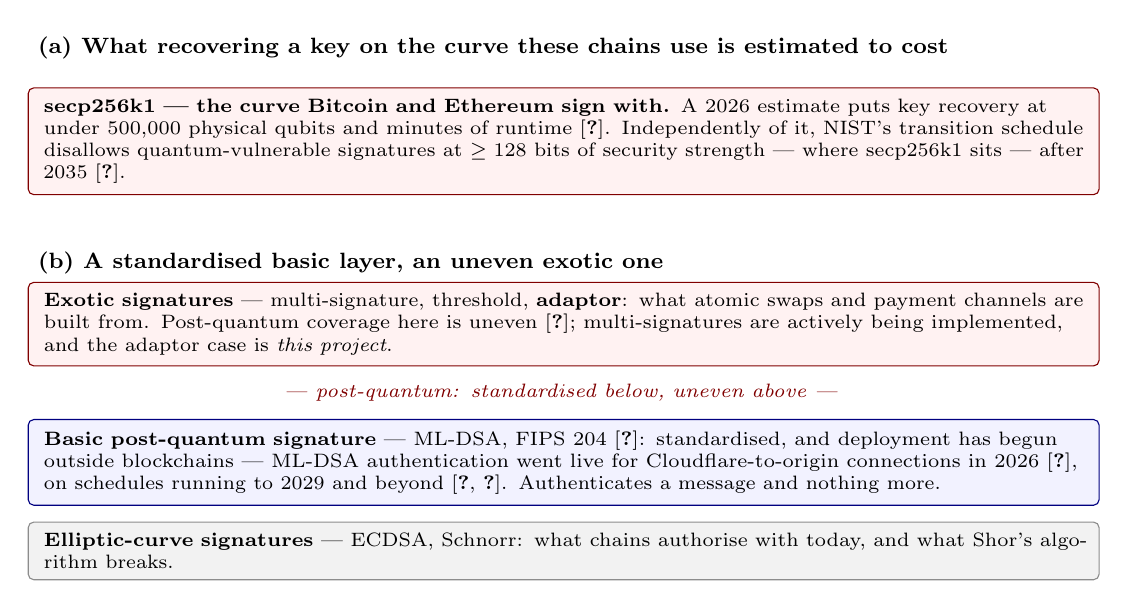
\begin{tikzpicture}[
      font=\scriptsize,
      ttl/.style={font=\footnotesize\bfseries, anchor=west},
      %% (an "est" style for the old three-column timeline lived here until the panel
      %% was rebuilt on 2026-08-27; it is referenced nowhere now)
      tier/.style={draw, rounded corners=2pt, align=left, text width=132mm,
                   inner xsep=2mm, inner ysep=1.4mm, anchor=north},
      gap/.style={font=\scriptsize\itshape, anchor=north, align=center,
                  text width=132mm}]

    %% Geometry: EVERY box is centred on x = 0 and the picture stays inside \textwidth
    %% (145mm).  Tier boxes span [-68mm, 68mm] (132mm text + 2mm inner xsep either
    %% side), and both panel titles are left-anchored at -68mm to match that edge.
    %% Keep it symmetric -- mixing left-anchored coordinates for (a) with centred ones
    %% for (b) once put the two halves on different axes and overran the text block.
    %% Vertical placement is RELATIVE (each row hangs off the previous one), so a row
    %% may grow in height without being edited into a collision.

    %% ---- (a) the estimated cost of breaking THE CHAINS' OWN curve ----
    %% Rebuilt 2026-08-27 (Meeting 12).  The earlier version was a three-dot timeline,
    %% two dots of which were RSA-2048; the supervisor read that as arguing from a
    %% target neither chain uses ("Bitcoin and also Ethereum, they are not using RSA")
    %% and asked for something "much closer to Bitcoin, or to blockchain itself".  The
    %% RSA figures are therefore REMOVED, not demoted.  Two consequences, both wanted:
    %% the panel now argues at secp256k1 only, and with no second target present there
    %% is no pair to divide, so the across-targets misreading is structurally gone.
    %% If any RSA figure is ever restored, the caption's separation caveat must come
    %% back with it -- and \cite{gidney2021factoring,gidney2025factoring} with it.
    %% WORDING: "the CURVE these chains use", never "the signature" -- they share
    %% secp256k1, not one scheme (Bitcoin has ECDSA and Schnorr).
    \node[ttl] at (-68mm,0) {(a) What recovering a key on the curve these chains use is
        estimated to cost};
    \node[tier, fill=red!5, draw=red!50!black] (pri) at (0mm,-5mm)
      {\textbf{secp256k1 --- the curve Bitcoin and Ethereum sign with.} A 2026 estimate
       puts key recovery at under 500{,}000 physical qubits and minutes of runtime
       \cite{babbush2026securing}. Independently of it, NIST's transition schedule
       disallows quantum-vulnerable signatures at $\ge 128$ bits of security strength
       --- where secp256k1 sits --- after 2035 \cite{nistir8547}.};
    \coordinate (bTop) at ([yshift=-6mm]pri.south);

    %% ---- (b) a standardised basic layer, an uneven exotic one ----
    %% NOT "standardisation stops": the cited claim is about the availability of
    %% practical IMPLEMENTATIONS, and multi-signatures are actively being built.
    %% Anchored to (a)'s last row via bTop, NOT to an absolute y: (a) may grow without
    %% the two halves colliding.
    \node[ttl, anchor=north west] at ([xshift=-68mm]bTop)
      {(b) A standardised basic layer, an uneven exotic one};
    \node[tier, fill=red!5, draw=red!50!black] (ex) at ([yshift=-5mm]bTop)
      {\textbf{Exotic signatures} --- multi-signature, threshold, \textbf{adaptor}:
       what atomic swaps and payment channels are built from. Post-quantum coverage
       here is uneven \cite{buser2023survey}; multi-signatures are actively being
       implemented, and the adaptor case is \emph{this project}.};
    \node[gap, red!50!black] (gp) at ([yshift=-1mm]ex.south)
      {--- post-quantum: standardised below, uneven above ---};
    %% NOT "being adopted now" unevidenced (the wording here until 2026-08-27, and the
    %% thing the supervisor asked for twice): deployment outside blockchains is CITED,
    %% and the live one is signature AUTHENTICATION on Cloudflare-to-origin connections
    %% -- never the public web PKI, where no post-quantum certificate was in use in 2025.
    \node[tier, fill=blue!5, draw=blue!50!black] (ba) at ([yshift=-1mm]gp.south)
      {\textbf{Basic post-quantum signature} --- ML-DSA, FIPS~204 \cite{1274601}:
       standardised, and deployment has begun outside blockchains --- ML-DSA
       authentication went live for Cloudflare-to-origin connections in 2026
       \cite{valenta2026pqauth}, on schedules running to 2029 and beyond
       \cite{cloudflare2026pqroadmap,nistir8547}. Authenticates a message and nothing
       more.};
    \node[tier, fill=black!5, draw=black!45] (ec) at ([yshift=-2mm]ba.south)
      {\textbf{Elliptic-curve signatures} --- ECDSA, Schnorr: what chains authorise
       with today, and what Shor's algorithm breaks.};
  \end{tikzpicture}
  \caption[Why now, and where the gap is]{Why the problem is timely, and where this
  project sits within it. \textbf{(a)} The case is made at the curve these chains
  actually sign with, secp256k1, rather than at a reference target neither of them
  uses. This is an estimate, for hardware nobody has built: what such work reports is
  the \emph{estimated cost of the attack}, not a calendar. The deadline beside it is
  independent of that estimate --- a policy schedule, which binds regardless of when
  the hardware arrives. \textbf{(b)} A
  blockchain does not rest on one signature but on a stack of them. The basic layer,
  which authenticates a message and nothing more, is standardised and being adopted;
  the functionality chains actually depend on lives in the exotic layer above it, where
  practical post-quantum coverage is uneven. That migration is not a blockchain concern
  alone, and it has run ahead on encryption: post-quantum key agreement already carried
  the majority of human traffic on one major network while no public post-quantum
  certificate was yet in use \cite{westerbaan2025pqinternet}, and post-quantum
  \emph{signatures} followed later --- ML-DSA authentication went live there for
  connections to origin servers in July 2026 \cite{valenta2026pqauth}, with full
  coverage targeted for 2029 \cite{cloudflare2026pqroadmap}. The basic signature layer
  is therefore the current frontier outside blockchains too. This dissertation addresses one scheme in
  that layer, the adaptor signature.}
  \label{fig:whynow}
\end{figure}

This dissertation focuses on the \emph{adaptor signature}, which ties the act of
publishing a valid signature to the simultaneous revelation of a secret witness
\cite{poelstra2017,aumayr2021generalized}. That property makes adaptor signatures useful
for scriptless blockchain protocols. In an atomic swap, revealing the witness on one leg
provides what is needed to complete the other, letting two parties exchange assets across
chains without a trusted intermediary (\cref{fig:swapidea}). They have also been applied to payment-channel
networks, linking conditional off-chain updates through the same
witness mechanism. Because the condition is embedded in the signature rather than
published separately, the result verifies as an ordinary signature and the condition need
not appear as a separate on-chain script \cite{esgin2020post,buser2023survey}. Existing
classical constructions rely largely on discrete-logarithm assumptions and so are not
post-quantum secure, while practical post-quantum implementations remain limited. That
combination --- important blockchain applications, and an implementation gap --- is why
the adaptor signature was selected from the exotic-signature family.

% MOVED HERE FROM ch:results 2026-08-27, after Meeting 12.  Wang reviewed the REPORT with
% the PDF on screen and named the adaptor motivation as the one substantive shortfall --
% "why is it important for blockchains?", "we need some concrete motivation, the concrete
% examples", "you should at least give some introduction regarding applications of the
% adaptor signature".  This figure is exactly that concrete example, so it belongs beside
% the claim it makes concrete rather than three chapters later.
%
% This does NOT disturb Meeting 10's ruling, which has two parts: Fig. 3.5 (fig:swapflow)
% is ACCEPTED and stays where it is -- it does, in ch:results -- and a simpler diagram goes
% "before it, where the application is introduced".  Both still hold: Chapter 1 precedes
% Chapter 3, and the application is now introduced HERE.  When M10 was given, it was
% introduced only in ch:results, because this chapter carried no atomic-swap material at
% all; that material is the Meeting-12 expansion above.
%
% Word cost is nil: a figure body and its caption are both excluded from the count, and the
% \cref added above is paid for by the one dropped from ch:results.
%
% PARTY NAMING IS SETTLED (2026-08-16) -- do not "fix" it either way.  The subscripts stay:
% this figure is the ONLY place Alice/Bob is tied to the u_1/u_2 the technical chapters use,
% and dropping them reintroduces exactly the inconsistency that decision removed.  What did
% not survive the move is the caption's old "used from here on", which was true when this
% figure sat in ch:results and is false here; the tie is restated neutrally instead.
%
% REDRAWN 2026-08-27 and the redraw MUST survive any future edit.  An earlier version drew
% one arrow from Alice to Bob and another back, with the ledgers reduced to words ON those
% arrows -- so the picture invited the reading that a coin travels from one chain to the
% other, which is false, and left the caption denying what the drawing showed.  The ledgers
% are the drawn objects now: each payment is a transaction sitting INSIDE its own lane.  Do
% not reintroduce a party-to-party coin arrow.  Absolute coordinates only -- no calc.
\begin{figure}[htbp]
  \centering
  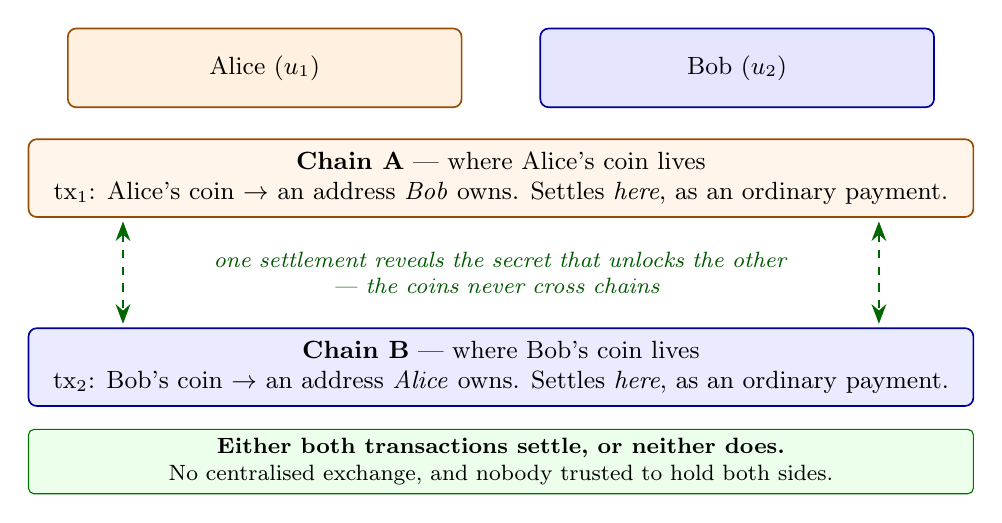
\begin{tikzpicture}[
      font=\small,
      party/.style={draw, rounded corners=3pt, align=center, minimum width=50mm,
                    minimum height=10mm, line width=0.6pt},
      lane/.style={draw, rounded corners=3pt, align=center, minimum width=120mm,
                   inner ysep=1.6mm, line width=0.6pt},
      lbl/.style={font=\footnotesize\itshape, align=center},
      >={Stealth[]}]

    \node[party, fill=orange!12, draw=orange!60!black] (a) at (30mm,0mm)
      {Alice $(u_1)$};
    \node[party, fill=blue!10, draw=blue!60!black] (b) at (90mm,0mm)
      {Bob $(u_2)$};

    \node[lane, fill=orange!8, draw=orange!60!black] (c1) at (60mm,-14mm)
      {\textbf{Chain~A} --- where Alice's coin lives\\
       $\mathrm{tx}_1$: Alice's coin $\rightarrow$ an address \emph{Bob} owns. Settles
       \emph{here}, as an ordinary payment.};

    % The link is drawn as two arrows FLANKING the label, so the label never covers the
    % thing it is labelling, and it is wrapped to stay inside the lane width.
    \draw[<->, dashed, line width=0.9pt, green!40!black] (12mm,-19.5mm) -- (12mm,-32.5mm);
    \draw[<->, dashed, line width=0.9pt, green!40!black] (108mm,-19.5mm) -- (108mm,-32.5mm);
    \node[lbl, green!35!black, text width=104mm] at (60mm,-26mm)
      {one settlement reveals the secret that unlocks the other\\
       --- the coins never cross chains};

    \node[lane, fill=blue!8, draw=blue!60!black] (c2) at (60mm,-38mm)
      {\textbf{Chain~B} --- where Bob's coin lives\\
       $\mathrm{tx}_2$: Bob's coin $\rightarrow$ an address \emph{Alice} owns. Settles
       \emph{here}, as an ordinary payment.};

    \node[draw, rounded corners=2pt, fill=green!8, draw=green!45!black,
          align=center, font=\footnotesize, minimum width=120mm] at (60mm,-50mm)
      {\textbf{Either both transactions settle, or neither does.}\\
       No centralised exchange, and nobody trusted to hold both sides.};
  \end{tikzpicture}
  \caption[An atomic swap, in outline]{What an atomic swap is for, before any
  cryptography --- one concrete blockchain application of adaptor signatures. Two parties
  want to trade coins that live on two different chains, and the danger is that one side
  takes payment and walks away. An atomic swap removes that danger: either both
  transactions settle or neither does, with no centralised exchange and nobody who has to
  be trusted to hold both sides. The two ledgers are drawn as the lanes because that is
  where the movement happens --- each payment settles as an ordinary transaction on its
  \emph{own} chain, so each party ends up holding an output on the other's ledger without
  any coin changing chain. What ties the two transactions together is secret information
  revealed by one settlement and used to unlock the other, not a transfer between chains;
  the parties also exchange several messages off-chain before either transaction is
  broadcast. Adaptor signatures provide the cryptographic link between the two settlements
  without requiring the swap condition to appear as a separate on-chain script. The two
  parties are named as in Esgin et al.\ \cite{esgin2020post}, whose $u_1$ and $u_2$ the
  later chapters use; \cref{fig:swapflow} sets the exchange out message by message.}
  \label{fig:swapidea}
\end{figure}

Cross-chain exchange first relied on custodial intermediaries; hash-time-locked contracts
removed the custodian by locking both transfers under one hash preimage, so claiming one
leg reveals the preimage unlocking the other. Such contracts, however, need explicit
on-chain script support, place a common hash on both chains --- linking the legs --- and
enlarge the transactions. Moving the lock into the signature answers all three
\cite{poelstra2017,aumayr2021generalized}: settlements look like ordinary single-signer
payments, atomicity is retained, and the witness reaches only the counterparty holding
the matching pre-signature. The link removed is the explicit protocol one; timing and
amounts can still correlate the legs.

\section{Subject area and related work}
\label{sec:relatedwork}

%% The "Exotic signatures for post-quantum blockchains" entry that stood here stated the
%% buser2023survey point a THIRD time (it is already made in sec:motivation and again in
%% the adaptor paragraph, both citing the same survey).  Removed 2026-08-27 to pay for
%% the expanded adaptor motivation Meeting 12 asked for; the citation is not lost.
\paragraph{Lattice signatures and Dilithium.}
CRYSTALS-Dilithium is a lattice signature in the ``Fiat--Shamir with aborts'' family
\cite{ducas2018crystals,lyubashevsky2012lattice}, its security reducing to the Module
Learning With Errors and Module Short Integer Solution problems. It samples a masked
commitment, derives a challenge by hashing, computes a response, and \emph{rejects and
retries} when the response would leak the secret --- the rejection-sampling step
characterising the family. Its reference implementation provides the polynomial
arithmetic, number-theoretic transform (NTT) and SHAKE-based sampling this project
reuses.

\paragraph{Adaptor signatures.}
Introduced informally as ``scriptless scripts'' \cite{poelstra2017} and later formalised
\cite{aumayr2021generalized}, the abstraction adds four algorithms to a base signature
--- \textsc{PreSign}, \textsc{PreVerify}, \textsc{Adapt}, \textsc{Extract} --- relative
to a hard relation $(Y,y)$: a pre-signature can be \emph{adapted} into a full signature
by anyone knowing the witness $y$, and publishing that signature lets anyone holding the
pre-signature \emph{extract} $y$. Anonymous multi-hop locks generalise this to payment
paths \cite{malavolta2019anonymous}.

\paragraph{Post-quantum adaptor signatures.}
Esgin, Ersoy and Erkin proposed LAS, a lattice-based adaptor signature on a
Dilithium-style base \cite{esgin2020post}; it is the design implemented here. Their work
is primarily theoretical --- definitions, a construction and security proofs --- leaving
the practical, benchmarked, blockchain-facing implementation open. poqeth studies how PQ
primitives are integrated and costed on Ethereum
\cite{kysil2025poqeth}, providing a template for the on-chain side.

\paragraph{Classical baseline.}
The natural answer to ``what does post-quantum cost'' is a comparison with a
\emph{classical adaptor} signature, not merely plain ECDSA. Mature ECDSA-adaptor
implementations exist \cite{secp256k1zkp}; this project benchmarks against one, stating
security parameters explicitly so the comparison is fair (\cref{ch:methodology}).

\section{Aim and objectives}
\label{sec:aims}

\paragraph{Aim.}
To implement and evaluate a post-quantum exotic signature scheme --- a lattice-based
adaptor signature reusing the CRYSTALS-Dilithium primitives --- and to demonstrate it
in a post-quantum blockchain atomic-swap application. The work is positioned as
\emph{systems implementation and evaluation}: it is grounded in existing cryptographic
research and does not propose a new cryptographic protocol.

\paragraph{Objectives.}
\begin{enumerate}
  \item Review post-quantum and exotic-signature literature sufficiently to justify
        selecting the adaptor signature LAS and the Dilithium primitives.
  \item Implement LAS additively on the Dilithium reference, reusing the lattice core
        unchanged and adding the adaptor operations and a byte-level wire encoding.
  \item Validate correctness and robustness through functional, serialization,
        tamper, and known-answer tests, including cross-validation by a second,
        independent implementation checked against the same known-answer digest.
  \item Benchmark LAS fairly --- at explicitly stated parameters, with repeated runs and
        reported variance --- against a simplified Dilithium baseline at identical
        parameters and a classical ECDSA-adaptor baseline, separating computation from
        communication cost across the five standard signature metrics.
  \item Demonstrate an end-to-end post-quantum atomic swap using the implementation
        --- following the protocol of \cite{esgin2020post}, including its
        zero-knowledge proof of knowledge $\pi$ --- and discuss its feasibility.
\end{enumerate}

\section{Contributions}
\label{sec:contributions}

This dissertation contributes a tested, independently cross-validated implementation of a
post-quantum adaptor signature, and measurements of its cost. Four findings carry it.
Adaptor functionality proves close to free in computation but expensive in communication:
its price is bytes, not time (\cref{sec:res-compute,sec:res-comm}). The design assertion the implementation rests on ---
that an adaptor needs an exact verification identity --- was tested, not argued, and proved
half wrong: \textsc{PreSign} and \textsc{PreVerify} must indeed be new algorithms, yet
an unmodified FIPS~204 verifier accepts the adapted signature (\cref{sec:res-mldsa}). At
application scale the bottleneck is not the signature but the zero-knowledge proof, leaving
the fully post-quantum swap the faster of the two such configurations and the only one Shor
does not break (\cref{sec:res-stage2}). And native on-chain verification, first
measured far above the transaction gas cap, fits under it once the same predicate is
re-expressed --- at the single parameter set and message length measured --- while a settled
swap sits well inside a UTXO chain's weight limit (\cref{sec:res-app,sec:res-txstruct}). All
five objectives were met (\cref{tab:objectives}), subject to two limits throughout: no
concrete security is formally analysed, and nothing ran on a live network.

\section{Dissertation structure}
\label{sec:structure}

\Cref{ch:methodology} describes the methods; \cref{ch:results} reports the measurements
and discusses their validity; \cref{ch:evaluation} judges the work against the
objectives; \cref{ch:conclusion} concludes, reflects critically, and proposes future
work.

\chapter{Methodology}
\label{ch:methodology}

\section{The LAS construction}
\label{sec:construction}

LAS is a lattice adaptor signature whose base is a simplified, Dilithium-style
Fiat--Shamir-with-aborts signature \cite{esgin2020post,ducas2018crystals}. All objects
live in $\Rq = \mathbb{Z}_q[X]/(X^d+1)$, the public matrix has the form
$A = [\,I_n \mid A'\,] \in \Rq^{\,n\times(n+\ell)}$, and a key pair is a short secret $r$
with its image $t = A\cdot r$. The hard relation $(Y,r')$ reuses exactly that structure,
% The hardness attribution follows the paper's own Section-3 hard-relation explanation,
% which is the M-SIS one.  The clause that stood here also credited M-LWE with "keeping the
% witness hidden": that is a security-analysis claim this project does not make, and the
% paper assigns M-LWE to the signature setting rather than to the relation.
so a statement is ``just another public key'': recovering a sufficiently short preimage of
$Y$ under $A$ is the Module-SIS problem underlying the relation's hardness
\cite{esgin2020post}. Esgin et al.\ \cite{esgin2020post}
name this statement-generation step \textsc{Gen}: sample an independent ternary vector
$r'$, compute $Y=A\,r'$, and
return $(Y,r')$. Thus \textsc{Gen} is not a further primitive but \textsc{KeyGen}
with its public key $t$ relabelled as the statement $Y$ and its secret $r$
relabelled as the witness $r'$. \emph{Key generation is shared}, so LAS is exactly the
base signature plus four adaptor operations. The implementation mirrors that split:
\texttt{relation\_gen} implements \textsc{Gen}, while \texttt{las.c} and
\texttt{las.rs} hold the adaptor layer alone.

The base signature commits to a mask $y$ as $w = A\,y$, forms a challenge
$c = H(\mathit{pk}, w, M)$, computes the response $\vecz = y + c\,r$ and rejects when
$\inftynorm{\vecz} > \gamma-\kappa$. Relative to a statement $Y$, the adaptor extension
\cite{esgin2020post} adds \textsc{PreSign}, which folds the statement into the hash,
$c = H(\mathit{pk}, w + Y, M)$, keeps the response $\hat{\vecz} = y + c\,r$, and rejects at
the \emph{tighter} bound
$\gamma-\kappa-1$; \textsc{PreVerify}, which recomputes $w' = A\hat{\vecz} - c\,t$ and checks
$c = H(\mathit{pk}, w'+Y, M)$; % NOT "$r' := y$": Algorithm 2 parses the pair that way, but this report reserves $y$ for
% the mask alone (see fig:flow's caption).  Writing the paper's local parse here made the
% sentence read as Adapt adding the masking randomness.
\textsc{Adapt}, which adds the witness $r'$,
$\vecz \leftarrow \hat{\vecz} + r'$, producing a signature the base verifier accepts; and
\textsc{Extract}, which recovers $s = \vecz - \hat{\vecz}$ (\cref{fig:lasfuncs}).

\begin{figure}[htbp]
  \centering
  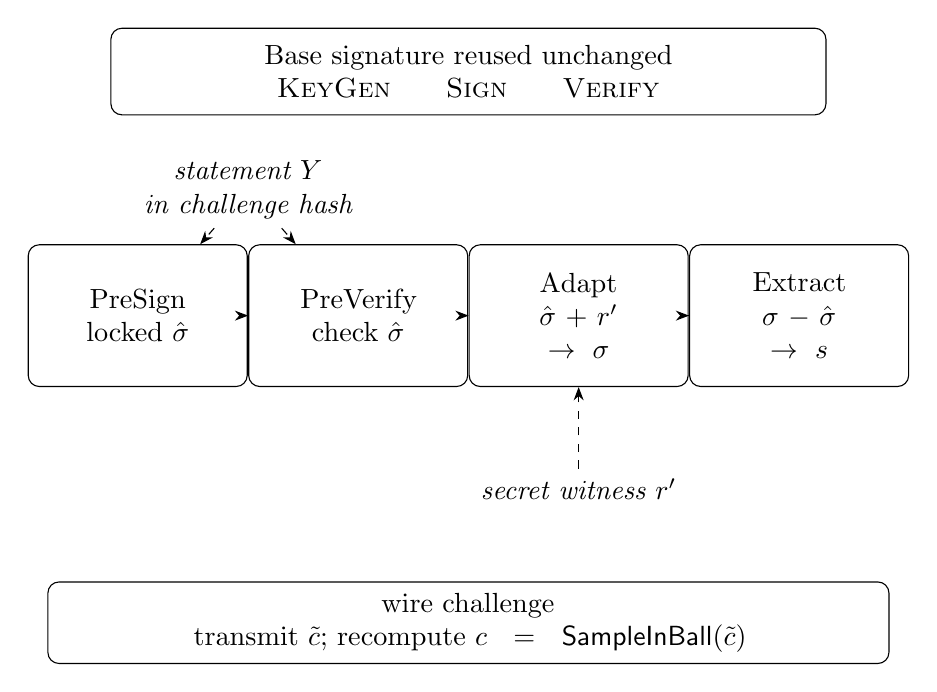
\begin{tikzpicture}[
      font=\normalsize,
      box/.style={draw, rounded corners, align=center, minimum height=11mm,
                  inner sep=4pt},
      base/.style={box, text width=88mm},
      opbox/.style={box, text width=25mm, minimum height=18mm},
      note/.style={font=\normalsize\itshape, align=center},
      wire/.style={box, text width=104mm, minimum height=10mm},
      >={Stealth[]}]

    \node[base] (base) at (0mm,0mm)
      {Base signature reused unchanged\\
       \textsc{KeyGen}\qquad \textsc{Sign}\qquad \textsc{Verify}};

    \node[opbox] (ps) at (-42mm,-31mm)
      {PreSign\\locked $\hat{\sigma}$};
    \node[opbox] (pv) at (-14mm,-31mm)
      {PreVerify\\check $\hat{\sigma}$};
    \node[opbox] (ad) at (14mm,-31mm)
      {Adapt\\$\hat{\sigma}+r'$\\$\to\sigma$};
    \node[opbox] (ex) at (42mm,-31mm)
      {Extract\\$\sigma-\hat{\sigma}$\\$\to s$};

    \draw[->] (ps) -- (pv);
    \draw[->] (pv) -- (ad);
    \draw[->] (ad) -- (ex);

    \node[note] (hash) at (-28mm,-15mm) {statement $Y$\\in challenge hash};
    \draw[->, dashed] (hash) -- (ps);
    \draw[->, dashed] (hash) -- (pv);

    \node[note] (wit) at (14mm,-53mm) {secret witness $r'$};
    \draw[->, dashed] (wit) -- (ad);

    \node[wire] at (0mm,-70mm)
      {wire challenge\\
       transmit $\tilde c$; recompute $c=\textsf{SampleInBall}(\tilde c)$};
  \end{tikzpicture}
  \caption[The four functions LAS adds to the base signature]{The four functions LAS
  adds around an unchanged base signature. \textsc{PreSign} and \textsc{PreVerify} bind
  the public statement $Y$ into the challenge; \textsc{Adapt} uses the witness $r'$ to
  turn the pre-signature into an ordinary signature; and \textsc{Extract} recovers a
  witness from that ordinary signature and the matching pre-signature. The implementation
  transmits $\tilde c$ and re-derives $c$ with \textsf{SampleInBall}.}
  \label{fig:lasfuncs}
\end{figure}

\begin{equation}
  \label{eq:signbound}
  \text{accept iff } \inftynorm{\vecz} \le \gamma-\kappa,
  \qquad \gamma = \kappa\, d\,(n+\ell).
\end{equation}

The subtle design point is the bound budget. An \emph{honest} witness is ternary, so
$\inftynorm{r'}\le 1$, and because \textsc{PreSign} rejects at $\gamma-\kappa-1$ the response
after \textsc{Adapt} clears \cref{eq:signbound}; loosening it to $\gamma-\kappa$ would let
adapted signatures exceed the bound and be rejected.
\Cref{fig:flow} shows the data flow.

\begin{figure}[htbp]
  \centering
  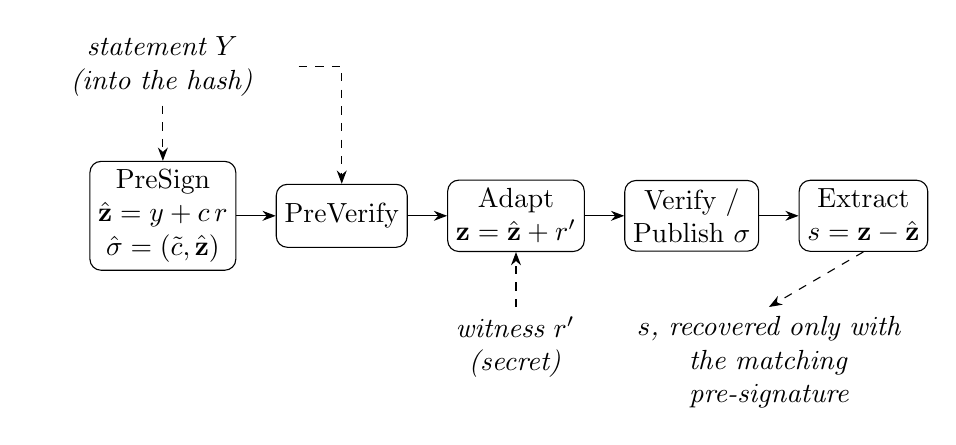
\begin{tikzpicture}[
      node distance=7mm and 5mm,
      box/.style={draw, rounded corners, align=center, minimum height=8mm,
                  inner sep=3pt, font=\normalsize},
      ann/.style={font=\normalsize\itshape, align=center, text width=32mm},
      >={Stealth[]}]
    \node[box] (ps)  {PreSign\\$\hat{\vecz}=y+c\,r$\\$\hat{\sigma}=(\tilde c,\hat{\vecz})$};
    \node[box, right=of ps] (pv) {PreVerify};
    \node[box, right=of pv] (ad) {Adapt\\$\vecz=\hat{\vecz}+r'$};
    \node[box, right=of ad] (vf) {Verify /\\Publish $\sigma$};
    \node[box, right=of vf] (ex) {Extract\\$s=\vecz-\hat{\vecz}$};
    \draw[->] (ps) -- (pv);
    \draw[->] (pv) -- (ad);
    \draw[->] (ad) -- (vf);
    \draw[->] (vf) -- (ex);
    % statement Y enters at PreSign and PreVerify (hashed into the challenge)
    \node[ann, above=of ps] (Y) {statement $Y$\\(into the hash)};
    \draw[->, dashed] (Y) -- (ps);
    \draw[->, dashed] (Y) -| (pv);
    % witness y enters at Adapt; is revealed by Extract
    \node[ann, below=of ad] (y) {witness $r'$\\(secret)};
    \draw[->, dashed] (y) -- (ad);
    % anchored to ex's right edge so the wrapped annotation grows leftwards and cannot
    % push the picture's bounding box past \textwidth at 12pt.
    \node[ann, text width=38mm, anchor=north east] (yo) at ([yshift=-7mm]ex.south east)
      {$s$, recovered only with\\the matching pre-signature};
    \draw[->, dashed] (ex.south) -- (yo.north);
  \end{tikzpicture}
  \caption[The LAS adaptor data flow]{The LAS adaptor data flow, in the symbols of
  \cref{fig:lasfuncs}: $y$ is PreSign's mask, $r'$ the honest witness, $s$ what Extract
  recovers. The statement $Y$ is folded into the challenge
  hash during PreSign and PreVerify; the witness is added by Adapt to turn the
  pre-signature into a base signature; and publishing that signature lets anyone
  holding the pre-signature run Extract to recover it. This last step is what an atomic
  swap uses.}
  \label{fig:flow}
\end{figure}

\section{Implementation strategy: reuse, do not reinvent}
\label{sec:impl}

The guiding principle is that an exotic scheme equals a basic scheme plus extra functions,
so the lattice arithmetic should be \emph{reused}, not rewritten. The implementation is
built additively on the upstream CRYSTALS-Dilithium reference
\cite{ducas2018crystals,pqcrystalsdilithium} at a pinned commit, and the same strategy is
applied again in Rust (\cref{sec:rustport}). Neither is itself ``the reference'': both are
\emph{modified, simplified} ML-DSA-style bases carrying the LAS layer of
\textcite{esgin2020post}.

Classifying every source file by how the reference is used (\cref{tab:reuse}) yields a
clean split: the entire lattice core is reused unchanged, while the adaptor scheme,
serialization, application integration, and evaluation harnesses are project-specific
additions. No upstream function is modified; the low-level Dilithium arithmetic and hash
primitives are reused unchanged. The vendored
\texttt{secp256k1-zkp} \cite{secp256k1zkp} and LaZer \cite{lazer} are unmodified too, the
latter behind a dedicated bridge.

\paragraph{Data types and the matrix product.}
LAS is a self-contained module over the reference's degree-$d$ polynomial type. Because
$A=[\,I_n\mid A'\,]$, the product $A\,v = v_{\text{top}} + A' v_{\text{bot}}$ multiplies only
$A'$.

\paragraph{Hash, challenge, and samplers.}
The random oracle $H$ is built from SHAKE256, absorbing a canonical encoding of the public
key, then the commitment ($w$ for Sign, $w+Y$ for PreSign), then the message. The challenge
sampler is the reference's \texttt{SampleInBall} at weight $\kappa$, giving
$\lVert c\rVert_1=\kappa$ and $\inftynorm{c}=1$. Two samplers are added: a ternary one for
secrets and witnesses, and a rejection sampler uniform on $[-\gamma,\gamma]$ for the mask
(\cref{app:methoddetail}).

\paragraph{Simplifications, and the modulus.}
Following \cite{esgin2020post}, the base signature omits Dilithium's hint vector,
Power2Round and high/low-bit decomposition, hashing the full commitment $w$ rather
than its high bits. This keeps the exact identity $A\vecz - c\,t = w$ available, at the cost of larger keys and
signatures. Whether those optimisations can coexist with an adaptor layer was not assumed
but \emph{tested} (\cref{sec:res-mldsa}). The modulus is reused too: the reference NTT fixes
$q=8\,380\,417\approx 2^{23}$, FIPS~204's own modulus \cite{1274601}, rather than the
$q\approx 2^{24}$ of \cite{esgin2020post} --- correctness is unaffected since
$q>2\gamma$, and only the Module-SIS/LWE margin differs. No module depends on a
mode-specific constant, so identical code runs at every parameter set.

\section{Serialization and the on-chain interface}
\label{sec:serialize}

A deployable scheme exchanges \emph{bytes}, not in-memory structs, so a bit-packed wire
encoding, a typed codec and a verify-from-bytes entry point were implemented.
Two decisions matter. Validation is \emph{asymmetric}: keys and witnesses are checked on
decode, a signature is not, so a tampered response is caught by Verify --- the entry
point the tamper test attacks. And, following FIPS~204
\cite{1274601}, a signature carries not the challenge polynomial $c$ but the digest
$\tilde c$ from which every consumer re-derives it, under the standard's $\lambda/4$ rule
(\cref{app:serialize}).

\section{Testing methodology}
\label{sec:testing}

Four test types cover progressively weaker assumptions about the environment, stated in
full in \cref{tab:tests}. Functional tests assume an honest caller and assert the whole
adaptor cycle, including the \emph{tripwire} clause --- a pre-signature must \emph{fail}
basic verification --- which is what distinguishes an adaptor signature from a signature.
Serialization and tamper tests assume a hostile caller; the known-answer test assumes a
different machine, and its digest is what the second implementation is checked against
(\cref{sec:rustport}).

\section{An independent second implementation: the Rust port}
\label{sec:rustport}

The complete scheme was implemented a second time in Rust on the same reuse principle,
layered on a fixed version of the \texttt{fips204} crate \cite{fips204crate}, with the LAS
layer added as new modules. The wire format is byte-identical to the C encoder's by
construction (\cref{fig:repostructure}).

\begin{figure}[htbp]
  \centering
  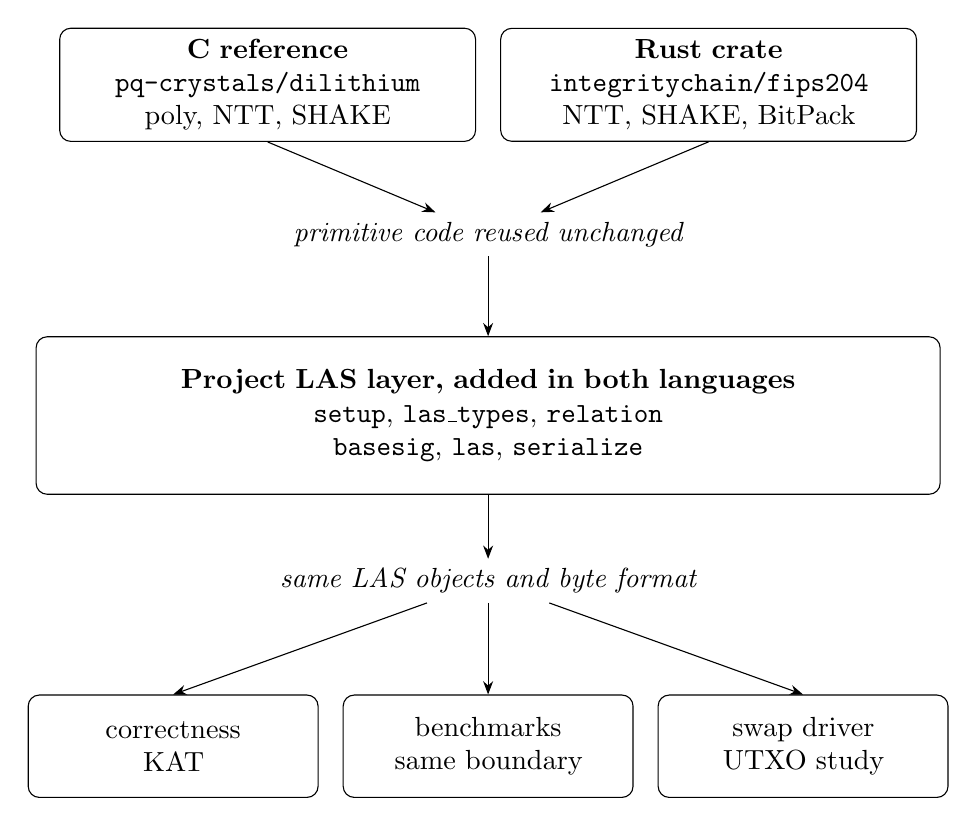
\begin{tikzpicture}[
      font=\normalsize,
      box/.style={draw, rounded corners, align=center, minimum height=11mm,
                  inner sep=4pt},
      source/.style={box, text width=50mm},
      layer/.style={box, text width=112mm, minimum height=20mm},
      evidence/.style={box, text width=34mm, minimum height=13mm},
      note/.style={font=\normalsize\itshape, align=center},
      >={Stealth[]}]

    \node[source] (csrc) at (-28mm,0mm)
      {\textbf{C reference}\\\texttt{pq-crystals/dilithium}\\
       poly, NTT, SHAKE};
    \node[source] (rsrc) at (28mm,0mm)
      {\textbf{Rust crate}\\\texttt{integritychain/fips204}\\
       NTT, SHAKE, BitPack};

    \node[note] (reuse) at (0mm,-19mm)
      {primitive code reused unchanged};
    \draw[->] (csrc.south) -- (reuse);
    \draw[->] (rsrc.south) -- (reuse);

    \node[layer] (laslayer) at (0mm,-42mm)
      {\textbf{Project LAS layer, added in both languages}\\
       \texttt{setup}, \texttt{las\_types}, \texttt{relation}\\
       \texttt{basesig}, \texttt{las}, \texttt{serialize}};
    \draw[->] (reuse) -- (laslayer.north);

    \node[note] (format) at (0mm,-63mm)
      {same LAS objects and byte format};
    \draw[->] (laslayer.south) -- (format);

    \node[evidence] (tests) at (-40mm,-84mm)
      {correctness\\KAT};
    \node[evidence] (bench) at (0mm,-84mm)
      {benchmarks\\same boundary};
    \node[evidence] (swap) at (40mm,-84mm)
      {swap driver\\UTXO study};
    \draw[->] (format) -- (tests.north);
    \draw[->] (format) -- (bench.north);
    \draw[->] (format) -- (swap.north);
  \end{tikzpicture}
  \caption[Implementation structure and C/Rust correspondence]{Implementation structure and
  C/Rust correspondence across the two implementations. C uses the vendored
  \texttt{pq-crystals/dilithium} reference \cite{pqcrystalsdilithium}, Rust uses the
  \texttt{integritychain/fips204} crate \cite{fips204crate}, and neither modifies
  upstream primitive functions. The project LAS layer is added in both languages with
  the same module split and packed object format; tests, known-answer vectors, matched
  benchmarks, and the UTXO swap driver are produced from that layer. The per-file
  classification is \cref{tab:reuse}.}
  \label{fig:repostructure}
\end{figure}

The port serves three purposes. \emph{Cross-validation}: short of a formal proof, the
strongest practical argument for correctness is a second implementation agreeing on pinned
vectors. \emph{An independent
benchmark methodology}: Criterion.rs \cite{criterionrs} shares no timing code with the C
harness, so agreement defends the C numbers against harness artefacts. \emph{Deployment
realism}: a memory-safe language is the plausible production vehicle.

To make the timings comparable the two protocol drivers mirror each other exactly ---
same repetition scheme, fixed seed, fixed message, success-path gating and rejection
statistics. One caveat qualifies the port's independence: where \cite{esgin2020post} leaves
an engineering choice open, Rust adopts the C implementation's, concretely an early-abort
rejection check. Sharing that is what makes the two languages time the same algorithm, but
it is established by inspecting the two norm checks rather than by the automated evidence,
which constrains outputs and rejection rates, not the work profile of a rejected attempt
(\cref{app:methoddetail}).

\section{Benchmarking methodology and fair comparison}
\label{sec:benchmethod}

The evaluation separates \emph{computation} cost (wall-clock time per operation) from
\emph{communication} cost (bytes transmitted or stored).

\paragraph{Measurement boundaries.}
Undocumented boundaries are a recognised benchmarking pitfall for lattice signatures
\cite{riou2026apples}, so every timing belongs to one of the three declared boundaries of
\cref{tab:tiers}: a \emph{core tier} isolating the adaptor algebra from encoding, a
\emph{packed tier} giving what an on-chain consumer pays, and, for the classical baseline
alone, the \emph{hybrid} boundary its library exposes. Comparisons are made only within one
boundary, and every base-versus-LAS comparison shows \emph{both}.


\paragraph{Implementation of record, repeatability, and machine.}
Unless a caption says otherwise, timings are the C implementation's, with the Rust results
reported separately and never averaged with them (\cref{tab:rust}). Every timing is a mean
$\pm$ sample standard deviation over the repetition scheme its caption states. All
non-random inputs are fixed, so variability comes only from rejection sampling and machine
noise, never from input selection \cite{riou2026apples}. Toolchain, hardware and per-table
commands: \cref{app:repro}.

\paragraph{Per-operation reporting, not cumulative.}
Every operation is timed independently: they are split across parties, so a combined figure
would average over costs never paid together and hide the per-operation overhead.

\paragraph{The primary comparison: LAS against its own simplified base.}
LAS is exactly its base signature plus four operations on the same code, parameters and
primitives, so every comparison holds all three fixed and varies only the adaptor layer
(justified in \cref{sec:eval-strategy}). Each adaptor operation is paired with the base
operation it mirrors --- \textsc{Adapt} against \textsc{Verify}, since it runs a
PreVerify before adding the witness --- and \textsc{Extract}, having no base analogue, is
reported separately.

\paragraph{Rejection sampling: the expected attempt count.}
Sign-class operations restart until the response passes its norm bound, so no timing claim
is meaningful without the attempt statistics. Each coefficient is accepted with probability
$\bigl(2(\gamma-\kappa)+1\bigr)/(2\gamma+1)$ \emph{independently of the secret} --- why the
response is simulatable (\cref{app:methoddetail}) --- and an attempt succeeds only if all
$(n+\ell)\,d$ pass:
\begin{equation}
  \label{eq:rejacc}
  p_{\mathrm{acc}}
  = \left(\frac{2(\gamma-\kappa)+1}{2\gamma+1}\right)^{(n+\ell)d}
  \approx \left(1-\frac{\kappa}{\gamma}\right)^{(n+\ell)d}
  \approx e^{-\kappa (n+\ell) d/\gamma} = e^{-1}\approx 36.8\%,
\end{equation}
the last step using the design choice $\gamma=\kappa\,d\,(n+\ell)$ from
\cite{esgin2020post}, made exactly so the expected number of restarts is ``about $e<3$''.
Expected attempts are $1/p_{\mathrm{acc}}$, and PreSign's bound being tighter by one, it is
\emph{expected} to restart slightly more often before any adaptor arithmetic is counted.

\paragraph{Rejection sampling: the run-validity gate.}
Because the attempt count is geometric, per-call timings are heavy-tailed and averages
over too few calls can drift several percent on rejection luck alone
\cite{riou2026apples}. The drivers therefore treat the attempt statistics as a
\emph{validity gate}: measured mean attempts must match the closed-form expectation within
five standard errors, and a failing run aborts instead of producing evidence. This is a
consistency check on the rejection rate, not a proof of sampler correctness
(\cref{app:methoddetail,app:benchalg}). A second gate precedes every timing: the
correctness contract is asserted on the objects about to be timed, so no failure path is
ever measured.

\paragraph{Parameter sensitivity and component sizes.}
To test whether the adaptor overhead scales with the lattice dimensions, the same
comparison is repeated at the four parameter sets of \cref{tab:params} (symbols in
\cref{tab:notation}). Each key and signature is decomposed into components, so the
\emph{cause} of a size difference can be identified, not merely its total stated.

\begin{table}[htbp]
  \centering
  \caption[Parameter sets used in the evaluation]{Parameter sets used in the evaluation. The \emph{LAS-2020/845 reference}
  set is \emph{paper-derived} rather than that paper's exact set: it takes the dimensions
  of \cite{esgin2020post}, a historical reference point corresponding to no ML-DSA set,
  but runs at this build's modulus, which the paper permits --- only the \emph{size} of
  $q$ matters, so the concrete value may be chosen for a fast NTT. The \emph{Simplified
  Dilithium-II/III/V} sets reuse the dimensions of Dilithium modes~2/3/5, aligning the
  reusable ML-DSA primitives and the challenge-digest strength $\lvert\tilde c\rvert$
  with ML-DSA-44/65/87 while retaining LAS's own ternary secret distribution, rejection
  bounds, exact hint-free relation and unoptimised serialization. They are engineering
  benchmark settings, \emph{not} formal NIST/ML-DSA security-equivalence claims: a
  matched dimension is not a claim that LAS \emph{is} the corresponding ML-DSA parameter
  set or inherits its security category. All lattice sets
  share the ring degree $d=256$ and modulus $q=8\,380\,417\approx 2^{23}$ inherited from
  the reused Dilithium NTT; \emph{Simplified Dilithium-III} is the project's target set.
  The classical secp256k1 ECDSA adaptor is a functionality-matched baseline at
  $\approx$128-bit classical security. \Cref{tab:notation} defines each symbol.}
  \label{tab:params}
  \small
  \setlength{\tabcolsep}{4pt}
  \begin{tabular}{@{}L{0.30\linewidth}rrrrrrr@{}}
    \toprule
    Setting & $n$ & $\ell$ & $M$ & $\kappa$ & $\gamma$ & $d$ & $q$ \\
    \midrule
    LAS-2020/845 reference            & 4 & 4 & 8  & 60 & 122\,880 & 256 & 8\,380\,417 \\
    Simplified Dilithium-II           & 4 & 4 & 8  & 39 & 79\,872  & 256 & 8\,380\,417 \\
    Simplified Dilithium-III (target) & 6 & 5 & 11 & 49 & 137\,984 & 256 & 8\,380\,417 \\
    Simplified Dilithium-V            & 8 & 7 & 15 & 60 & 230\,400 & 256 & 8\,380\,417 \\
    \midrule
    Classical (secp256k1 ECDSA adaptor)
      & \multicolumn{7}{c}{$\approx$128-bit classical (see \cref{tab:classical})} \\
    \bottomrule
  \end{tabular}
\end{table}


\paragraph{The classical baseline: functionality-matched, not security-matched.}
The second baseline is the \texttt{secp256k1-zkp} library's \texttt{ecdsa\_adaptor}
module \cite{secp256k1zkp}, implementing Fournier's construction
\cite{fournier2019adaptor}, unmodified at a pinned commit. It is a functionality-matched
``price of post-quantum'' baseline, not a same-security one; plain ECDSA is excluded, the
fair counterpart of an adaptor signature being another adaptor signature.

\section{Application methodology: the UTXO swap study}
\label{sec:stage2method}

This section defines the application protocol and the measurement boundary used for the
Stage-2 results. The protocol follows Figure~1 of Esgin, Ersoy and Erkin
\cite{esgin2020post} over two UTXO ledgers; \cref{sec:res-app} later reports the execution
evidence, while \cref{sec:res-stage2,sec:res-txstruct} report cost.

\paragraph{The venue, and why it is modelled.}
The construction \cite{esgin2020post} states its applications over ``a UTXO-based
blockchain like Bitcoin \emph{where the signature algorithm is replaced with a
lattice-based signature scheme}''. That sentence is implemented literally: a UTXO ledger
was built in which \emph{the signature algorithm is a parameter}, so one ledger serves
every configuration and any measured difference is the cryptography, not the ledger. It is
a model, not a node; the boundary is set out in \cref{app:utxomodel}.

\paragraph{The protocol that is executed.}
\Cref{fig:swapflow} is the run book implemented by the driver. Alice, written $u_1$ in the
paper notation, holds the witness $y$ and therefore moves first; Bob, written $u_2$, only
pre-signs after the proof $\pi$ and Alice's pre-signature have both verified. That proof is
part of the method, not decoration: it proves the statement has a short witness, closing
the knowledge gap that would otherwise let a malicious first party leave an unadaptable
pre-signature behind. Operationally, a pre-signature is only a wallet-to-wallet protocol
message: no UTXO is spent while $\hat{\sigma}_i$ is being exchanged. A blockchain event
occurs only when an adapted signature is placed in the transaction's ordinary signature
field and that transaction is broadcast to its own ledger. The other ledger never verifies
a foreign transaction; atomicity comes from Bob observing $\sigma_2$ on ledger~B, extracting
the witness, and using it to finish the spend on ledger~A.

\begin{figure}[htbp]
  \centering
  % Type is \normalsize throughout: nothing inside a figure may be smaller than the
  % body text.  The geometry below was re-derived for 12pt -- widths from the longest
  % line in each box, row pitch from the tallest box -- so do not shrink the font back
  % to fit a coordinate.
  % The ledger boxes say "verifies $\sigma_i$", NEVER "validates witness": this report
  % uses "witness" for the secret $y$, which is never transmitted, so that wording read
  % as the ledger checking an object it never sees.
  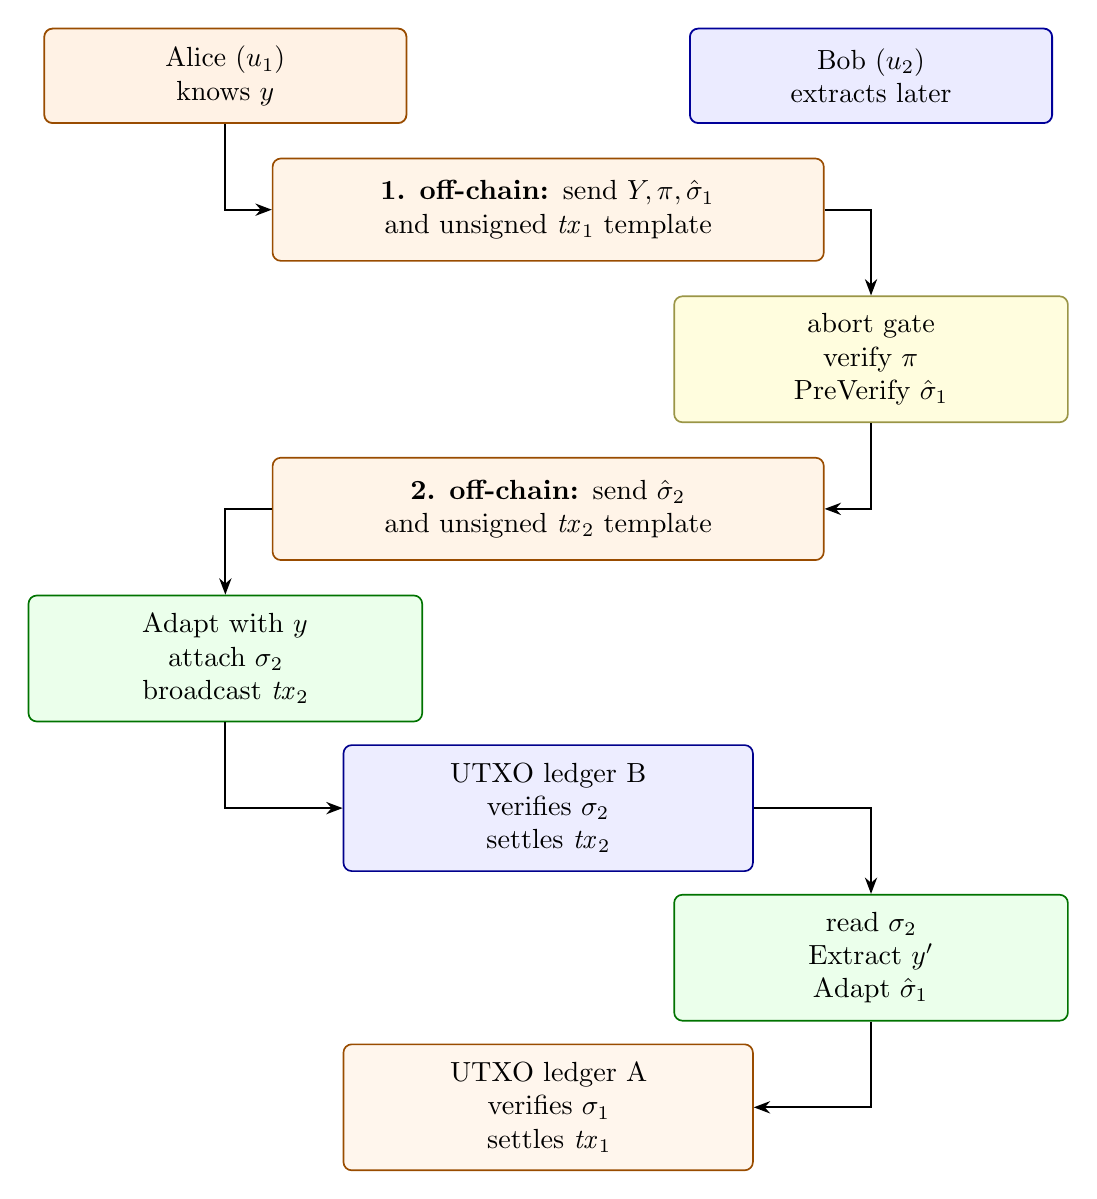
\begin{tikzpicture}[
      font=\normalsize,
      party/.style={draw, rounded corners=3pt, align=center, minimum width=46mm,
                    minimum height=12mm, line width=0.65pt},
      msg/.style={draw, rounded corners=3pt, fill=orange!9, draw=orange!60!black,
                  align=center, text width=68mm, minimum height=13mm,
                  inner xsep=1mm, inner ysep=1mm, line width=0.6pt},
      gate/.style={draw, rounded corners=3pt, fill=yellow!13, draw=yellow!55!black,
                   align=center, text width=48mm, minimum height=16mm,
                   inner xsep=1mm, inner ysep=1mm, line width=0.6pt},
      chain/.style={draw, rounded corners=3pt, fill=blue!7, draw=blue!55!black,
                    align=center, text width=50mm, minimum height=16mm,
                    inner xsep=1mm, inner ysep=1mm, line width=0.6pt},
      >={Stealth[]}]

    \node[party, fill=orange!10, draw=orange!60!black] (u1) at (24mm,0mm)
      {Alice $(u_1)$\\knows $y$};
    \node[party, fill=blue!8, draw=blue!60!black] (u2) at (106mm,0mm)
      {Bob $(u_2)$\\extracts later};

    \node[msg] (m1) at (65mm,-17mm)
      {\textbf{1. off-chain:} send $Y,\pi,\hat{\sigma}_1$\\
       and unsigned $\mathit{tx}_1$ template};
    \node[gate] (check) at (106mm,-36mm)
      {abort gate\\verify $\pi$\\PreVerify $\hat{\sigma}_1$};
    \draw[->, line width=0.65pt] (u1.south) |- (m1.west);
    \draw[->, line width=0.65pt] (m1.east) -| (check.north);

    \node[msg] (m2) at (65mm,-55mm)
      {\textbf{2. off-chain:} send $\hat{\sigma}_2$\\
       and unsigned $\mathit{tx}_2$ template};
    \draw[->, line width=0.65pt] (check.south) |- (m2.east);

    \node[gate, fill=green!8, draw=green!45!black] (adapt2) at (24mm,-74mm)
      {Adapt with $y$\\attach $\sigma_2$\\broadcast $\mathit{tx}_2$};
    \draw[->, line width=0.65pt] (m2.west) -| (adapt2.north);

    \node[chain] (chain2) at (65mm,-93mm)
      {UTXO ledger B\\verifies $\sigma_2$\\settles $\mathit{tx}_2$};
    \draw[->, line width=0.65pt] (adapt2.south) |- (chain2.west);

    \node[gate, fill=green!8, draw=green!45!black] (extract) at (106mm,-112mm)
      {read $\sigma_2$\\Extract $y'$\\Adapt $\hat{\sigma}_1$};
    \draw[->, line width=0.65pt] (chain2.east) -| (extract.north);

    \node[chain, fill=orange!7, draw=orange!60!black] (chain1) at (65mm,-131mm)
      {UTXO ledger A\\verifies $\sigma_1$\\settles $\mathit{tx}_1$};
    \draw[->, line width=0.65pt] (extract.south) |- (chain1.east);
  \end{tikzpicture}
  \caption[The atomic-swap protocol used in the UTXO study]{The atomic-swap protocol used
  in the UTXO study, adapted from Figure~1 of \cite{esgin2020post}. Only the two adapted
  signatures reach ledgers, inside the ordinary signature/witness field of their own
  transactions; $Y$, $\pi$, the unsigned templates and the pre-signatures are off-chain
  protocol messages, and the witness $y$ is never transmitted. Step~1 gives Bob enough
  evidence to decide whether to continue; step~2 gives Alice the pre-signature she can
  adapt with $y$; once $\sigma_2$ is visible in the settled transaction on ledger~B, Bob
  extracts $y'$ and adapts the first leg for ledger~A.
  The signed message $m_i$ is the signature hash of the unsigned template
  $\mathit{tx}_i$, not the transaction bytes themselves. \Cref{sec:res-app} reports the
  assertions that this flow passed, and \cref{sec:res-stage2} measures its cost.}
  \label{fig:swapflow}
\end{figure}
\FloatBarrier

\paragraph{What a settled transaction contains, and what the adaptor layer changes.}
Of the adaptor-protocol objects exchanged by
the swap, only the adapted signature $\sigma$ reaches a ledger, occupying the slot in
which an ordinary signature already appears --- since SegWit
\cite{bip141}, a segregated \emph{witness} field. The statement $Y$, the proof $\pi$ and
both pre-signatures stay off-chain, while the witness $y$ is never transmitted: $u_2$
derives it from the published $\sigma$ and its own pre-signature. The construction
therefore adds \emph{no adaptor-specific on-chain field} --- what \emph{scriptless}
means: the swap condition need not appear as a separate on-chain script. The resulting
transaction cost is obtained by mapping the measured signature-scheme objects onto the
fields of \cite{bip141,bip144,bip341} --- signature and public key into the witness, the
committed key hash into the output script --- accepting that mapping only once it
reproduces published reference sizes for an ordinary spend (\cref{sec:res-txstruct}).

One notational point matters once the venue is a real ledger. The swap protocol writes the
signed object as $\mathit{tx}_i$, but a transaction is not a message: a signature commits to
its \emph{signature hash}. Three objects are therefore kept distinct --- the unsigned
template exchanged off-chain, its signature hash (the message passed to \textsc{PreSign}),
and the settled transaction --- since conflating them would misreport communication cost.

\paragraph{Three configurations, and what is controlled.}
The three configurations of \cref{tab:configs} each run the swap protocol end-to-end
across two ledgers. The \emph{role-A} proof is the proof of knowledge $\pi$ the protocol
places on the wire immediately after $Y$, claiming a witness to $Y$ exists and is short.
Only the $2\to3$ step is controlled: both LAS configurations share one expansion of the
public matrix, derive all key material from one pinned seed, and prove the
\emph{identical} relation
$\exists\, r' : A r' = t' \wedge \inftynorm{r'} \le 1$ --- the hard relation of the
statement/witness pair, \emph{not} the signer's key pair, and including the norm bound,
since proving only $A r' = t'$ would fail to close the knowledge gap. This is verified
rather than assumed: a configuration whose two halves disagree on a \emph{relation
binding} each computes independently refuses to run (\cref{app:methoddetail}).
The $1\to2$ step is not controlled --- it changes the signature scheme, the relation and
whether a role-A proof exists --- so it is a whole-stack comparison, the signature-only
question being answered by \cref{sec:res-classical}.

\begin{table}[htbp]
  \centering
  \caption[The three measured configurations]{The three configurations. Only the
  $2\to3$ step is controlled: those two share one public matrix, prove the identical
  relation, and receive byte-identical inputs from one pinned seed, so their difference
  is the proof system alone. Configuration~1 carries \emph{no} role-A proof, and this
  is a finding rather than an omission: LAS needs $\pi$ because of its knowledge gap
  --- extraction returns a witness of the extended relation, which need not be ternary,
  so without $\pi$ a malicious $u_1$ could claim and leave $u_2$ holding an unadaptable
  pre-signature --- whereas an ECDSA adaptor has no such gap, since extraction recovers
  the discrete logarithm exactly. The measured \texttt{secp256k1-zkp} construction
  accordingly carries no $\pi$, and adding one would have measured a modified baseline
  rather than the library as it stands. The DLEQ proof
  carried \emph{inside} a \texttt{secp256k1-zkp} pre-signature is a different object
  and is not counted as $\pi$: its author is the pre-signer, and its claim is
  pre-signature well-formedness, not knowledge of the role-A statement witness $r'$.
  Its cost is reported in the bytes by which a pre-signature exceeds a signature.}
  \label{tab:configs}
  \small
  \begin{tabular}{@{}lL{0.27\linewidth}L{0.30\linewidth}cc@{}}
    \toprule
    \# & Signature & Role-A proof $\pi$ & Setup & Fully PQ \\
    \midrule
    1 & \cfgOneSigName{}   & \cfgOnePiName{}   & ---         & \cfgOneFullyPQ{} \\
    2 & \cfgTwoSigName{}   & \cfgTwoPiName{}   & trusted     & \cfgTwoFullyPQ{} \\
    3 & \cfgThreeSigName{} & \cfgThreePiName{} & transparent & \cfgThreeFullyPQ{} \\
    \bottomrule
  \end{tabular}
\end{table}

\paragraph{The Groth16 circuit.}
No pairing-based proof of this lattice statement was available to reuse, so the circuit is
new, and cheaper than the statement suggests: $r' \mapsto A r'$ is \emph{linear with public
coefficients}, needing no witness--witness multiplication, the expensive ingredient in a
rank-one constraint system (\cref{app:methoddetail}).

\paragraph{Measurement.}
Because gas does not exist on this venue, the axes are execution time and communication
cost, the latter counting \emph{off-chain} protocol messages, not only what reaches a
ledger. Sizes are observed from the transmitted buffers rather than computed, and these
timings sit at the \textbf{packed tier}, so they are not comparable with core-tier figures
elsewhere. One-time costs are excluded and reported separately (\cref{app:methoddetail}).

\chapter{Results and discussion}
\label{ch:results}

This chapter reports what was built and measured, and discusses why the results
should be believed. It covers correctness testing, then computation cost, then
communication cost with the component breakdown, and finally the application
demonstration.

\section{Correctness and robustness}
\label{sec:res-correctness}

Before any performance claim, the implementation must be shown to be \emph{correct}.
An adaptor signature is not correct merely because it signs and verifies; it must
satisfy a specific contract, and a consolidated harness (\texttt{test\_contract})
checks every clause of that contract and prints each as a labelled pass. \Cref{tab:contract}
lists the checks and their outcomes.

\begin{table}[t]
  \centering
  \caption{The adaptor-signature correctness contract, each clause checked and passed
  by \texttt{test\_contract} (corroborated at scale by the 1000-iteration functional
  suite on modes 2/3/5, the 256-instance serialization suite, and the pinned
  known-answer test).}
  \label{tab:contract}
  \begin{tabular}{@{}llc@{}}
    \toprule
    \# & Property & Result \\
    \midrule
    1 & PreSign produces a pre-signature that PreVerify accepts & pass \\
    2 & the pre-signature \emph{fails} basic Verify (statement-binding tripwire) & pass \\
    3 & Adapt yields a signature that basic Verify accepts & pass \\
    4 & Extract recovers the witness \emph{exactly} ($y'=y$) & pass \\
    5a & a tampered message fails Verify & pass \\
    5b & every single bit-flip of the packed signature is rejected & pass \\
    6 & malformed packed bytes are rejected ($pk\!\ge\!Q$, ternary code-3, $z$ out of band) & pass \\
    7 & the deterministic API is byte-identical on re-run & pass \\
    \bottomrule
  \end{tabular}
\end{table}

Each clause matters. Clauses~1--4 are the adaptor contract itself: a pre-signature is
verifiable yet unspendable (the tripwire, clause~2), becomes a basic signature
once the witness is added (clause~3), and the act of completing it reveals the witness
(clause~4) --- the mechanism that makes an atomic swap atomic. Clauses~5--6 are
robustness: the byte-level verifier an on-chain integration would consume must not
trust its input, so it rejects tampering and malformed encodings. Clause~7 is
reproducibility, which lets an independent verifier be cross-checked against fixed
vectors. All clauses pass, with zero compiler warnings under the project's strict
flags.

\section{Computation cost}
\label{sec:res-compute}

The primary, fair comparison is LAS against its own simplified base, since they share
algorithm, parameters, and primitives (\cref{sec:benchmethod}); it measures the
overhead of the adaptor layer. \Cref{tab:overhead} reports it at the project's target
setting, \emph{Simplified Dilithium-III} ($n{=}6$, $\ell{=}5$, $\kappa{=}49$;
\cref{tab:params,tab:notation}), pairing each adaptor operation with the basic
operation it mirrors; \cref{tab:overhead-levels} then confirms the same overhead at all
four settings. Each entry is the mean $\pm$ sample standard deviation over ten runs of
one thousand iterations (\texttt{bench\_levels}).

\begin{table}[t]
  \centering
  \caption{Key overhead summary at the \emph{Simplified Dilithium-III} (target) setting
  ($n{=}6$, $\ell{=}5$, $M{=}11$, $\kappa{=}49$, $\gamma{=}137\,984$, $N{=}256$,
  $q{=}8\,380\,417$); $\mu$s/op, mean $\pm$ sample SD over 10 runs $\times$ 1000
  iterations (\texttt{bench\_levels}). Overhead is each adaptor operation over its basic
  analogue; KeyGen (and statement generation) is shared by the basic signature and LAS.}
  \label{tab:overhead}
  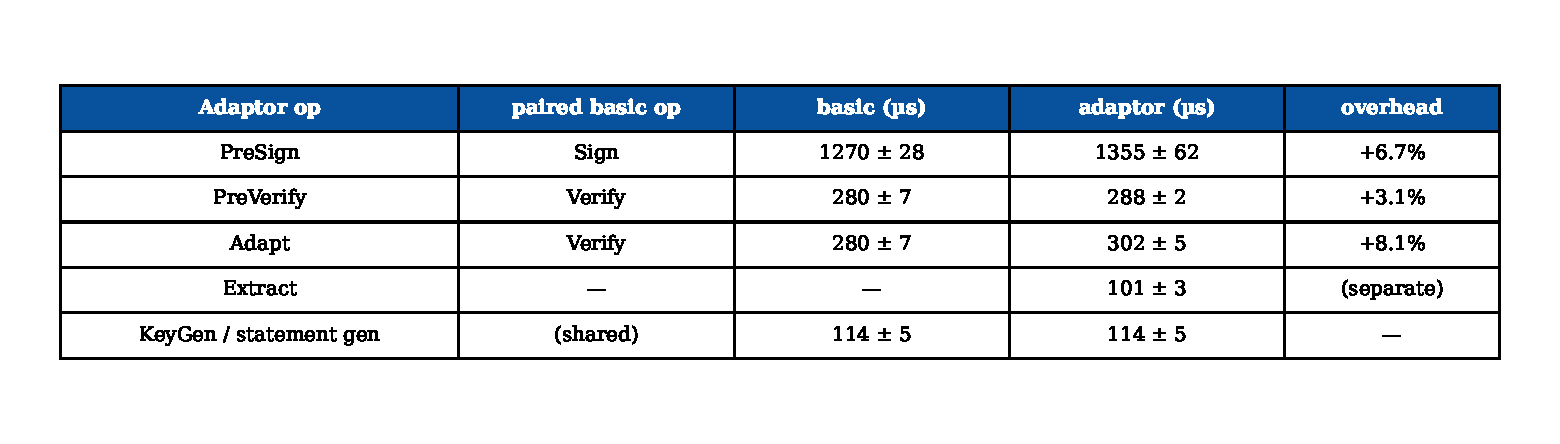
\includegraphics[width=0.9\linewidth]{figures/tab_overhead_l3}
\end{table}

The result is that the adaptor layer is almost free in computation, and the numbers
are not just small --- they are small \emph{for structural reasons}:
\begin{itemize}
  \item \textbf{PreSign $\approx$ Sign} ($+6.7\%$): PreSign runs the same masked-commit,
        hash, respond, reject loop as Sign; it only adds the statement $Y$ into the
        Fiat--Shamir commitment and rejects at a slightly tighter bound. Neither
        changes the asymptotic work.
  \item \textbf{PreVerify $\approx$ Verify} ($+3.1\%$): PreVerify recomputes the same
        commitment shape as Verify, differing only by the $+Y$ addition before hashing.
  \item \textbf{Adapt $\approx$ Verify} ($+8.1\%$): Adapt first runs a PreVerify and
        then adds the witness vector, so it costs about one verification plus a few
        polynomial additions.
  \item \textbf{Extract is cheapest and reported separately}: it has no basic analogue;
        it only subtracts $z-\hat z$ and checks $A\,y=Y$.
\end{itemize}

This overhead is stable across security levels. \Cref{tab:overhead-levels} repeats the
measurement at each parameter set: the adaptor premium stays in the single digits ---
at most about eight percent --- everywhere, so adding adaptor functionality does not
become more expensive as the scheme is scaled up.

\begin{table}[t]
  \centering
  \caption{Adaptor overhead is small at every parameter set (\texttt{bench\_levels};
  mean over 10 runs $\times$ 1000 iters, Extract in $\mu$s). Percentages are each
  adaptor operation over its basic analogue.}
  \label{tab:overhead-levels}
  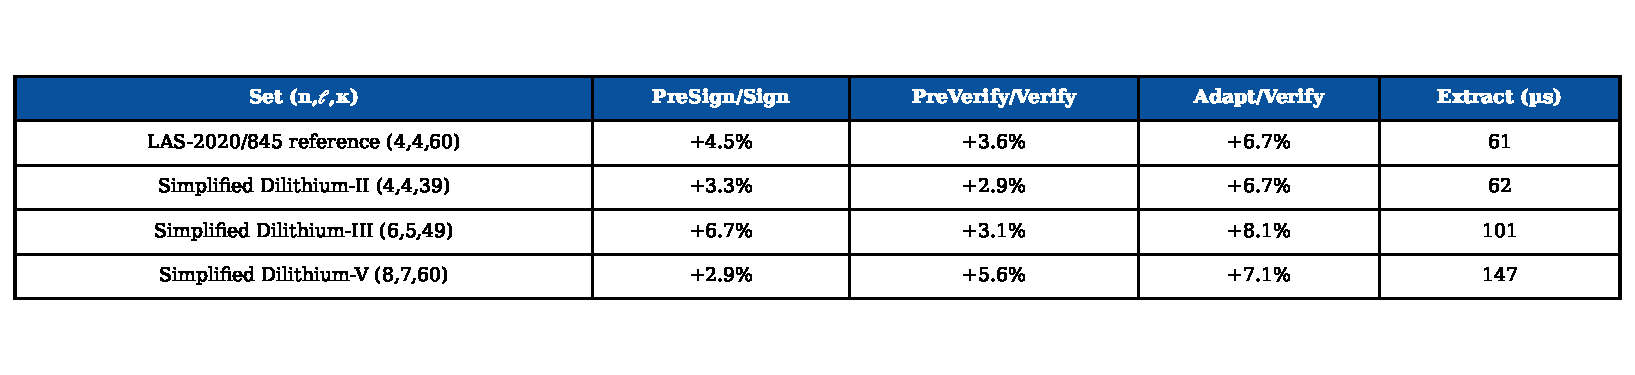
\includegraphics[width=\linewidth]{figures/tab_overhead_levels}
\end{table}

Signing and pre-signing are dearer than verification because they use rejection
sampling. The acceptance rate was measured directly, by counting rejection-loop
attempts rather than estimating from a timing ratio: at every setting approximately
37\% of attempts are accepted, so a signature takes about 2.7 attempts on average. This matches the closed-form prediction: one attempt is accepted only if
all $(n+\ell)\cdot N$ response coefficients fall within the bound, giving a per-attempt
acceptance of $(1-\kappa/\gamma)^{(n+\ell)N}\approx e^{-1}\approx 36.8\%$. Rejection
sampling is intrinsic to the Fiat--Shamir-with-aborts family, not a defect of this
implementation.

\section{Communication cost and component breakdown}
\label{sec:res-comm}

The computation results above show the adaptor layer is cheap. The size results show
where the real cost lies. \Cref{tab:components} decomposes every LAS object into its
components, in actual packed bytes (by the field-width formula the serializer uses),
across the parameter sets. The aim is to explain \emph{which} component drives the
size, not merely to state that signatures are large.

\begin{table}[t]
  \centering\small
  \caption{LAS objects by component (packed bytes; \texttt{bench\_levels}). The
  LAS-2020/845 reference set shares the Simplified Dilithium-II dimensions. The
  challenge $c$ is fixed; the response $z$ grows with $n+\ell$ and dominates the
  signature at every setting.}
  \label{tab:components}
  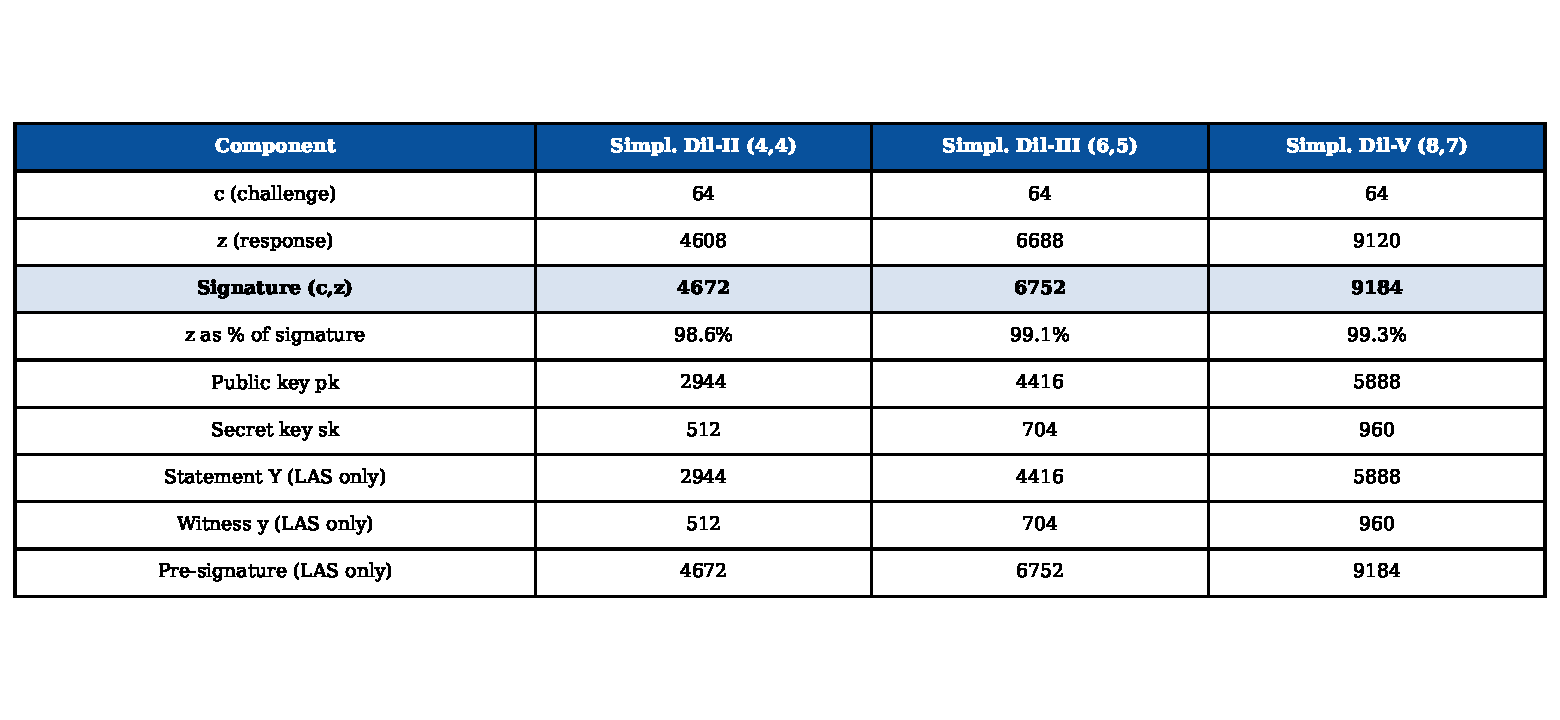
\includegraphics[width=0.85\linewidth]{figures/tab_components}
\end{table}

Two points follow, and together they give the sharp conclusion of the evaluation:
\begin{itemize}
  \item \textbf{The response $z$ is essentially the entire signature} --- 98.6\% at
        Simplified Dilithium-II, rising to 99.3\% at Simplified Dilithium-V. The
        challenge $c$ is a fixed 64 bytes and
        is irrelevant to size. Any optimisation of LAS signatures is an optimisation
        of $z$.
  \item \textbf{An adaptor swap additionally transmits a public-key-sized statement
        $Y$ and a signature-sized pre-signature}, while the witness is small. These are
        the only objects an adaptor protocol sends that a basic signature does not.
\end{itemize}

\noindent\textbf{The sharp conclusion: the cost of LAS is not adaptor computation but
communication --- specifically the response vector $z$ and the statement $Y$.} The
preceding section showed the adaptor operations add at most about eight percent of
compute over the basic scheme; this section shows the objects that move on the wire are
one to a few kilobytes, dominated by $z$. For a blockchain setting, where every byte is
stored and replicated, this is the property that matters, and it is a far more useful
statement than ``the signature is 4672 bytes''.

The response is stored at its full width: each coefficient occupies 18--19 bits
(\cref{tab:components}) rather than being range-reduced or entropy-coded. This is the
clearest opportunity for reducing the on-wire footprint, since compressing $z$ would
shrink the signature, pre-signature, and settlement payload together; it is left as
future work (\cref{sec:future}).

For a single reference point, \cref{tab:complete-l3} consolidates \emph{every}
communication object and \emph{every} protocol operation at the target setting next to
the basic signature, so the complete cost of the adaptor layer can be read in one
place: the key pair and KeyGen are shared, the four adaptor operations add single-digit
time overhead, and the only extra objects on the wire are the public statement $Y$ and
the signature-sized pre-signature.

\begin{table}[t]
  \centering\small
  \caption{Complete LAS vs.\ basic-signature comparison at the \emph{Simplified
  Dilithium-III} (target) setting ($n{=}6$, $\ell{=}5$, $M{=}11$, $\kappa{=}49$,
  $\gamma{=}137\,984$, $N{=}256$, $q{=}8\,380\,417$). \emph{Top:} communication ---
  packed bytes of every object. \emph{Bottom:} computation --- $\mu$s/op, mean $\pm$
  sample SD over 10 runs $\times$ 1000 iterations (\texttt{bench\_levels}). ``Basic'' is
  the simplified Dilithium-style base signature; shared rows are byte- or
  cycle-identical in both. The adapted signature is itself a valid basic signature.}
  \label{tab:complete-l3}
  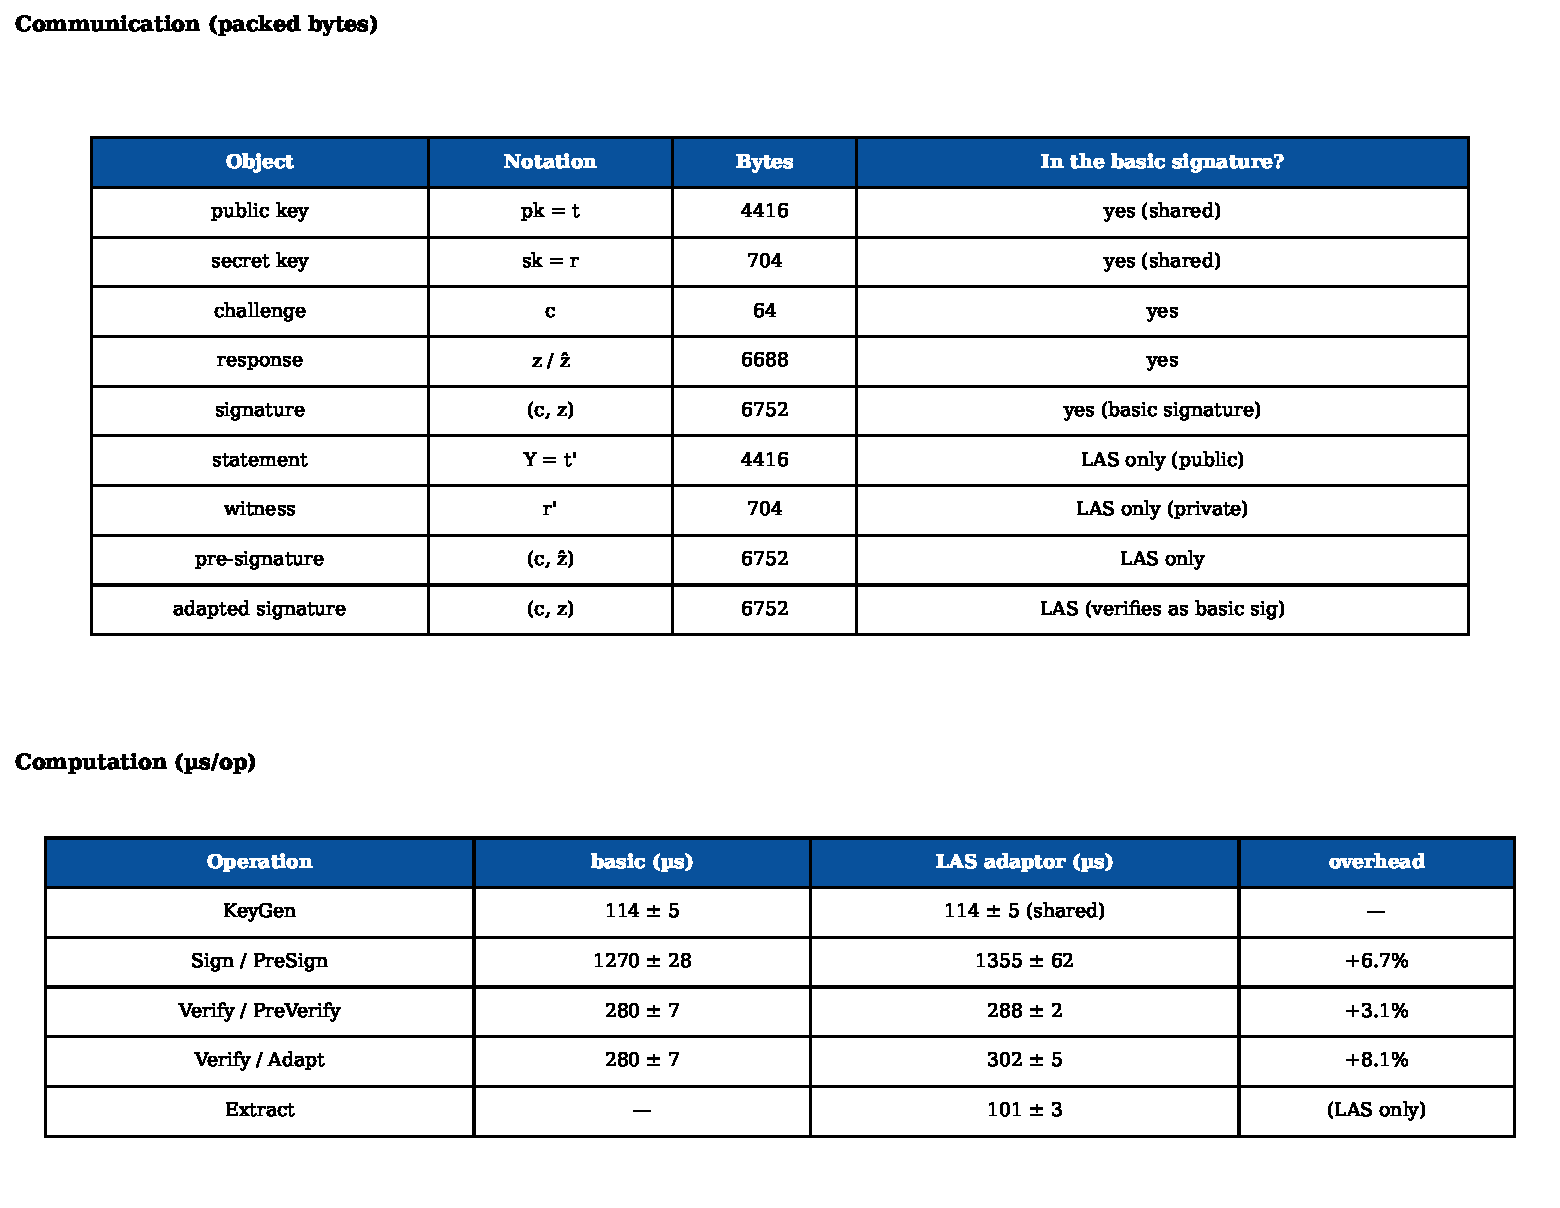
\includegraphics[width=0.95\linewidth]{figures/tab_complete_l3}
\end{table}

\subsection{The price of post-quantum: classical adaptor baseline}
\label{sec:res-classical}

The second baseline is a classical secp256k1 ECDSA adaptor signature
\cite{secp256k1zkp}. It is the natural functional counterpart of LAS: both are adaptor
signatures with the same operation set (KeyGen, Sign, Verify, PreSign, PreVerify,
Adapt, Extract) and both drive scriptless atomic swaps. They are compared on equal
footing functionally, while differing in their security foundation: secp256k1 provides
approximately 128-bit \emph{classical} security and is not quantum-resistant, whereas
LAS rests on lattice assumptions believed to resist quantum attack. The comparison
therefore measures the practical cost of moving from a classical adaptor signature to a
post-quantum one. Plain ECDSA is not used, because the counterpart of an adaptor
signature is another adaptor signature.

For this baseline LAS is instantiated at the \emph{Simplified Dilithium-II} parameters,
and only that setting is used. The reason is that secp256k1 offers roughly 128-bit
classical security, and the nearest post-quantum target is NIST level~2 (also pitched at
the 128-bit category); aligning LAS to the Dilithium-II dimensions therefore gives the
most like-for-like security target for the classical scheme. Comparing the 128-bit
classical adaptor against LAS at the Simplified Dilithium-III or -V settings would pit
it against a deliberately stronger post-quantum configuration and would understate the
classical scheme, so the higher settings are reserved for the parameter-sensitivity
study of \cref{sec:res-compute} and not used here. \Cref{tab:classical} reports both
schemes at their adaptor operations.

\begin{table}[t]
  \centering
  \caption{Classical vs.\ post-quantum adaptor signature: same functionality, different
  security foundation. Classical secp256k1 ($\approx$128-bit classical) and LAS at the
  \emph{Simplified Dilithium-II} parameters. Timings $\mu$s/op (mean over 10 runs
  $\times$ 1000 iterations, same machine); sizes in bytes. KeyGen also produces the
  statement/witness, which take the public-key/secret-key size.}
  \label{tab:classical}
  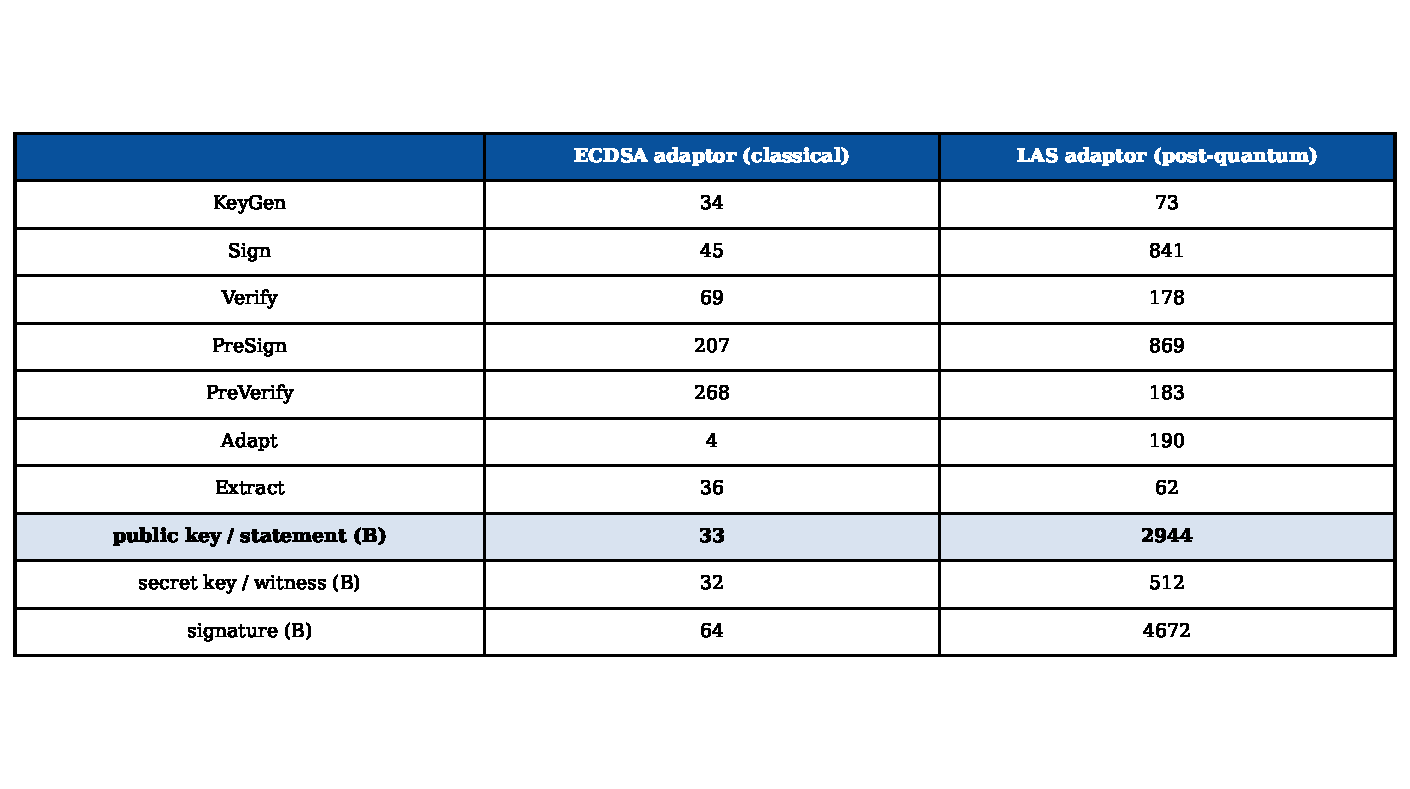
\includegraphics[width=0.72\linewidth]{figures/tab_classical}
\end{table}

This baseline compares two adaptor-signature schemes with the same high-level
functionality but different security assumptions: classical discrete-log security
versus post-quantum lattice security. Two findings stand out. First, the post-quantum
price is paid almost entirely in \emph{size}: LAS's public key and signature are
roughly 70 to 90 times larger than the classical adaptor's, whereas the operation times
differ by at most about twenty times and stay sub-millisecond. Second, the two schemes
pay their
\emph{adaptor} overhead in opposite ways. The classical ECDSA adaptor must attach a
discrete-logarithm-equality proof, so its PreSign and PreVerify are several times its
own basic sign and verify; LAS folds the statement into a hash it already computes, so
its adaptor operations stay within a few percent of its base operations. In
computation, then, the lattice adaptor layer is relatively cheaper to add than the
classical one; the post-quantum cost surfaces in communication, consistent with the
component analysis above.

\section{Application demonstration}
\label{sec:res-app}

The implementation was demonstrated in an end-to-end post-quantum atomic swap. Two
parties, Alice and Bob, swap coins across two ledgers with no trusted third party and
no on-chain scripts. Bob draws a fresh statement/witness pair $(Y,y)$ and sends only
$Y$. Each party pre-signs its outgoing transaction against the \emph{same} $Y$ and
checks the other's pre-signature; at this point neither pre-signature is spendable.
Bob, who knows $y$, adapts and publishes his signature to claim Alice's coin; the act
of publishing reveals $y$, which Alice extracts and uses to adapt and publish her own
signature, claiming Bob's coin. Either both legs settle or neither does. The demo
prints this narrative and asserts every step, including the counterfactual that a
pre-adaptation signature fails basic verification.

A small ledger abstraction takes this closer to a real chain: accounts with balances,
a block height, and adaptor-locked contracts (the scriptless analogue of a
hash-time-locked contract, with the hash lock replaced by the statement $Y$ and the
time lock by a timeout height). Three scenarios are asserted: a cross-chain swap
(happy path), a timeout/refund path in which a premature refund is rejected and both
parties recover their funds after the timeout, and a multi-hop payment.

As a bonus-tier check on deployability, the byte-level verifier was also costed on a
real Solidity stack: a native on-chain LAS verification measures at approximately
12 million gas, about 40\% of Ethereum's 30 million per-block limit. It therefore
fits within a block, though at a cost that motivates the precompile or
zero-knowledge-proof routes discussed in \cref{sec:future}. This on-chain measurement
and the multi-hop variant are bonus-tier evidence; they support, but do not displace,
the first-stage signature results above.

\section{Threats to validity}
\label{sec:res-validity}

Several factors qualify the results, and are stated here so the reader can judge how
far to trust them. First, all timings are machine-dependent; this is mitigated by
reporting the standard deviation, fixing one machine and compiler, and emphasising
ratios over absolute values. Second, the LAS parameter set's concrete security level
is not formally established, because security proofs are out of the project's scope;
every cross-scheme size and speed claim is therefore qualified by the explicit
parameters in \cref{tab:params}, and the fair comparison deliberately holds parameters
fixed between LAS and its simplified-Dilithium base. Third, the modulus is
$q\approx 2^{23}$, inherited from the reused NTT table, rather than the paper's
$2^{24}$; correctness is unaffected ($q>2\gamma$) but the security margin differs.
Fourth, the extracted witness is exact in this parameterisation, whereas the paper's
relaxed setting allows witness noise that can grow across long payment-channel paths;
the exact-extraction choice sidesteps that growth for the demonstration but is a
simplification worth noting.

\chapter{Evaluation}
\label{ch:evaluation}

\section{Evaluation strategy and its justification}
\label{sec:eval-strategy}

% "The aim" collided with sec:aims, which states a broader project aim.  This is the
% evaluation question, not the project aim, and the two must not share a name.
The project set out to measure what adaptor functionality \emph{costs}, so the evaluation
was built around one requirement: every measured difference had to have a single
attributable cause. Four decisions follow from it.

Correctness comes before cost. Performance figures for an incorrect implementation are
worthless, and no formal proof was in scope, so correctness rests principally on
differential evidence: a pinned known-answer value reproduced byte for byte by a second,
independently written implementation. Internal self-consistency is not enough, and one
error described below left every primitive passing in isolation while the assembled whole
was wrong.

The primary comparison is controlled. LAS is measured against its own simplified base at
identical algorithm, parameters and primitives, so the paired difference estimates the
cost of the adaptor layer and of nothing else. Measuring against optimised
CRYSTALS-Dilithium instead would confound that cost with parameter, packing and
hint-vector differences; that contrast is therefore kept only as context, and the
classical ECDSA adaptor only as a functionality-matched price of post-quantum.

% NOT "two tiers": sec:benchmethod declares THREE boundaries -- core, packed, and the
% hybrid one the classical library exposes.  The warrant for "misleads quietly" is local
% ("twice here"), never a general claim about benchmarking.
Every measurement declares its boundary, because an undeclared boundary misleads quietly,
as it did twice here before the tiers were fixed. For the same reason each run gates a
directly counted rejection rate against its closed-form prediction rather than inferring
acceptance from a timing ratio.

Metrics follow the venue. The application study reports execution time and communication
bytes, counting off-chain messages, because the evaluated UTXO ledger carries no gas
metric and because off-chain messaging is where the post-quantum cost lands.

\section{Achievement of the objectives}
\label{sec:eval-objectives}

\begin{table}[htbp]
  \centering
  % ⚠ This table is referenced from 01-introduction.tex ("All five objectives were met"),
  % so tab:objectives must not be deleted: doing so leaves a dangling \cref in Chapter 1,
  % which is also why the caption no longer repeats that verdict.  Its pointers ARE the
  % point of it -- a marker without the repository needs to know where each claim is
  % evidenced -- so the row text is what compresses, never the references.
  \caption[Objectives against evidence]{Each objective of \cref{sec:aims} against the
           evidence for it, which spans the introduction, \cref{ch:results} and the
           appendix.}
  \label{tab:objectives}
  \begin{tabular}{@{}p{0.24\textwidth}p{0.68\textwidth}@{}}
    \toprule
    \textbf{Objective} & \textbf{Evidence} \\
    \midrule
    1. Literature and scheme selection
      & Adaptor signature chosen for its direct relevance to atomic swaps; LAS
        \cite{esgin2020post} for the shortest path from a standardised lattice signature
        (\cref{sec:relatedwork}). \\[3pt]
    2. Additive implementation
      & Lattice core reused byte-for-byte with no upstream function modified, audited by
        a two-branch diff; adaptor layer, wire encoding and application are new code
        (\cref{tab:reuse}). \\[3pt]
    3. Validation
      & Functional, serialization, tamper and known-answer tests pass
        (\cref{sec:res-correctness}); an independent Rust implementation reproduces the
        wire format and the pinned value byte-for-byte (\cref{sec:res-rust}). \\[3pt]
    4. Fair benchmarking
      & Adaptor overhead isolated per operation at two declared tiers
        (\cref{tab:overhead-l3}), against two further baselines, with the rejection rate
        gated against theory and the relative conclusions reproduced by the Rust port
        (\cref{tab:rust}). \\[3pt]
    5. Atomic-swap demonstration
      & End-to-end two-party, two-chain swap settling both legs and asserting
        unspendability before adaptation (\cref{sec:res-app}), extended to a measured
        three-configuration study on a UTXO ledger (\cref{sec:res-stage2}). \\
    \bottomrule
  \end{tabular}
\end{table}

% SCOPE: only configurations 2 and 3 share one public matrix and byte-identical inputs
% (backend.rs "configurations()": one LasParams, hence one A, key material from one master
% seed).  Configuration 1 is secp256k1 and has no lattice matrix at all, so an unscoped
% sentence claims a control the study does not have -- sec:res-stage2 says "only the 2->3
% step is controlled" on its own page.
% PAGINATION: pulls one line from the next page back onto this one, so the section
% heading that follows is not left with only two lines beneath it.  This paragraph
% begins on that page, which is where \enlargethispage takes effect.
% ⚠ Pagination-dependent -- re-check on rebuild.
\enlargethispage{\baselineskip}
Fairness was not simply asserted. The standalone evaluation holds algorithm, parameters
and primitives fixed; in the application study the step from Groth16 to LaZer shares one
public matrix and byte-identical inputs, verified at run time, while the classical
configuration rests on a different curve and is a whole-stack contrast rather than a
controlled one. The figures are then defended from two independent directions: a
closed-form gate on the rejection rate, and re-measurement under a different compiler and
an independent statistical harness. That second check is also where the claims stop.
Absolute per-operation times do not reproduce across the two implementations and are not
offered as a comparison between them; what reproduces, and what the conclusions rest on,
is the relative cost of the adaptor layer.

% tab:onchain's own caption says its rows are --gas-report CHARGES, "not transaction
% totals and not client measurements", so setting the figure straight against a
% per-transaction cap conflates the two accounting boundaries that caption separates.
The demonstration was built in the UTXO setting assumed in \cite{esgin2020post}, then
measured against a gas-metered venue for contrast. There a \emph{complete}, validated
native LAS verifier was charged $\approx$\gasLasVerifiedM{} million gas for its claim
path, beyond the EIP-7825 per-transaction cap, though that figure is a
% "bound the IMPLEMENTATION rather than the scheme" is an equivalence claim, and the
% equivalence holds only under the registration invariant no contract checks (tab:onchain),
% which is why that reference stays: without it the caveat has no warrant in this chapter.
% The single instance belongs here too: two verifier stages branch on coefficient values.
\texttt{--gas-report} charge rather than a transaction receipt. The cap turned out to
bound the \emph{implementation} rather than the scheme: a restructured verifier was mined
by a real client inside it, at the target parameter set, for the message length and single
signature instance measured, and only under the registration invariant that
\cref{tab:onchain} records as unchecked. The venue decision rests on cost, not on
impossibility.

\section{Implementation challenges}
\label{sec:eval-challenges}

% REWRITTEN 2026-09-06 as continuous synthesis.  The previous version framed the section
% around "the six problems of tab:challenges" and three recurring themes; both were
% scaffolding rather than content, and the cross-reference made a body section depend on an
% appendix table (now deleted).  Each challenge is stated as problem -> why it resisted
% ordinary debugging -> fix, and every reference points at a main chapter.
%
% ⚠ SCOPES THAT MUST NOT DRIFT, each corrected during drafting:
%  - NOT "all four adaptor operations still succeed": app:challenges named THREE (PreSign,
%    PreVerify, Extract).  "the adaptor operations can still succeed" avoids the count.
%  - NOT "no local test observes it": an unbounded universal.  Scope it to the tests run.
%  - NOT "restores the adaptor properties" for ML-DSA: that experiment is a FUNCTIONAL
%    demonstration only and the security of committing to HighBits(w+Y) is unanalysed, so
%    the claim is scoped to the tested contract.
%  - NOT "the known-answer value exposed divergences": its purpose is cross-checking, and
%    nothing on record says it caught a specific divergence.  Say what it made possible.
%  - ORDER: the Solidity error was found by comparing the recomputed challenge digest
%    against the C reference; correction, then stagewise validation, then the gas-cap
%    restructuring followed.  Stagewise validation must not be named as what exposed it.
%  - The patched rule's SECURITY is unanalysed (a caveat that never lapses).  It is carried
%    here by "experimental" plus sec:res-txstruct, whose own prose states it in full.
\textsc{PreSign} must reject at $\gamma-\kappa-1$, one tighter than \cref{eq:signbound}.
At the looser bound the adaptor operations can still succeed while the adapted signature
later exceeds the norm ordinary \textsc{Verify} accepts; local adaptor tests did not expose
it, and accounting for the witness norm identified the tighter bound. A related assumption,
that Dilithium's hint and bit-splitting optimisations had to be disabled, also proved too
strong: carrying the commitment path on $w+Y$ satisfies the tested adaptor contract with
them enabled (\cref{sec:res-mldsa}).

Implementing the scheme independently in Rust required byte-identical agreement, including
deterministic sampling and serialization; the pinned known-answer value made that agreement
directly testable (\cref{sec:rustport}). Benchmarking raised a separate problem, because
rejection sampling makes sign-class timings right-skewed: acceptance inferred from a timing
ratio was biased, and the two timed loops initially performed unequal work. Attempts are
therefore counted directly, checked against theory, and measured at declared boundaries
(\cref{sec:benchmethod}).

The Groth16 circuit initially cloned growing linear combinations while constructing dense
rows, making the work quadratic in row width; building each row once through the
lower-level constraint interface reduced it to linear cost. In Solidity, an
already-NTT-domain public matrix was transformed again, producing a verifier that disagreed
with the C reference; comparing the recomputed challenge digest against C exposed the
error, the corrected port was validated in stages, and the verifier was then restructured
to fit the per-transaction gas cap (\cref{sec:res-evm}). Bitcoin imposed different
constraints: Script has no native lattice-signature verifier, and its \btcChunkWidth\,B
element limit prevents LAS signatures and public keys from being supplied as single
elements. The integration therefore chunks these objects and reassembles them inside an
experimental patched consensus rule (\cref{sec:res-txstruct}).

\section{Limitations}
\label{sec:eval-limitations}

% "three", not "two": the ZKNox dependency below is the third.  It was previously carried
% only in the deleted app:challenges caption, and it scopes a MEASURED gas figure, so it
% belongs in the body rather than an appendix (2026-09-06).
The threats of \cref{sec:res-validity} bound what the results \emph{mean}, and three further
limitations belong to the artefact itself, not to the measurement. The EVM verifiers reuse
lattice primitives from a library its authors describe as not production-ready, so the gas
figures characterise a numerically-correct verifier rather than a deployable one. The
hint-free
construction yields larger keys and signatures than optimised Dilithium: cryptographic
optimisation traded for a transparent and testable artefact. \Cref{sec:res-mldsa}
quantifies that price and shows it recoverable in principle, but only for the signature
and not for the statement.

% NOT "not a stack anyone should deploy": a normative absolute the evidence does not
% carry.  What is supported is that it is not fully post-quantum.
Configuration~2 gives up something different. Groth16's soundness rests on a pairing
assumption Shor breaks, so a post-quantum signature does not protect a swap whose fairness
rests on a classical proof. That configuration is the intermediate point which makes the
controlled proof-system comparison possible, and is reported as that and nothing more.

\chapter[Conclusion and future work]{Conclusion, critical reflection, and future work}
\label{ch:conclusion}

\section{Conclusions}
\label{sec:conclusions}

The aim was met within the prototype scope declared for it. The lattice core is reused
unchanged; the adaptor layer, the wire encoding and the application are new and tested;
functional, serialization, tamper and known-answer tests pass; a second implementation
reproduces the pinned value byte for byte; and a two-party, two-chain swap runs end to
end.

What adaptor functionality costs over a plain signature, and what a post-quantum operation
costs over a classical one, are answered with measured data at declared boundaries. Over
its own simplified base at identical parameters, the adaptor layer adds $+\ovPreSign\%$,
$+\ovPreVerify\%$ and $+\ovAdapt\%$ for PreSign, PreVerify and Adapt at the core tier,
staying within $+\ovMaxAll\%$ across the parameter sweep and reaching
$+\packedOvPreSign$--$\packedOvAdapt\%$ once the wire codec is counted, the increase there
being codec work rather than arithmetic. Communication is where the cost actually falls:
the signature is \zPctTarget\% response vector, with the statement $Y$ on top of it. The
classical comparison points the same way from the other side, its
discrete-logarithm-equality proof making that adaptor layer proportionally the more
expensive of the two.

The implementation follows the simplified Dilithium-style base of \cite{esgin2020post}, and
rebuilding the adaptor path on ML-DSA showed that the simplification is not functionally
required for final verification. \textsc{PreSign} and \textsc{PreVerify} do need
% "at equal computation" would overstate sec:res-mldsa, whose measured finding is that
% per-signature cost is "close to equal": ML-DSA restarts about twice as often, each
% attempt costing roughly half.  The hedge is the finding, so it travels with the claim.
adaptor-specific algorithms, since the naive port fails outright, but \textsc{Verify} does
not: a standard FIPS~204 verifier accepts the adapted signature. That route would halve the
signature at close to equal computation and leave $Y$ untouched: the communication bottleneck would move to the statement, not disappear.

Taking the protocol to the UTXO setting assumed in \cite{esgin2020post} sharpens the
conclusion. At application scale the signature is not the dominant cost at all: the role-A
proof consumes \cfgTwoProofPct\% of a Groth16 swap and \cfgThreeProofPct\% of a LaZer one.
Changing only the proof system makes the fully post-quantum swap \cmpTimePctAbs\% faster
end to end and \cmpBytesPctAbs\% larger in communication; it needs no trusted setup and is
the only one of the two Shor does not break, paying for that in bytes and in slower proof
verification. The principal qualification is scope: no concrete security is formally
analysed, and nothing settled on a live network.

\section{Critical reflection}
\label{sec:reflection}

\subsection{What was achieved}
\label{sec:reflection-achieved}

The decision that shaped everything else was additive construction on a standardised reference, with no lattice arithmetic reimplemented. It made the implementation tractable
and its provenance auditable: the security-critical arithmetic is byte for byte the
published CRYSTALS-Dilithium reference, and a two-branch diff shows exactly what was added.
Being language-agnostic, that decision also made the second implementation cheap, which
turned self-consistency into cross-implementation evidence and exposed the timing
conclusions to an independent harness. Pairing a pinned known-answer value with an
independent reimplementation proved a decisive way to validate a cryptographic port.

Two things went better than expected. Comparing LAS with its parameter-matched simplified
base separated the adaptor overhead from the cost of Dilithium's omitted optimisations,
which is the comparison every headline figure depends on. And counting rejection attempts
rather than inferring them from timing corrected a materially wrong earlier figure; it is
now a gate every run must pass.

% ⚠ "Compressing the statement", not narrowed to truncation: sec:future closes BOTH
% candidates -- truncation is fatal at both boundaries, and the seed candidate succeeds but
% hands over the witness -- so compressing Y inside this construction is closed outright.
% Narrowing it to truncation alone would understate what was measured.
Two negative results are worth as much. Compressing the statement inside this construction,
and proving the relation under a succinct post-quantum system, were both implemented and
neither paid off. Each now names the mechanism that defeats it, which closes the first
direction outright and the second at the scale measured here.

\subsection{What fell short}
\label{sec:reflection-shortfalls}

Three shortfalls remain beyond the scoped limitations of \cref{sec:eval-limitations}.

% ⚠ ACCOUNTING BOUNDARY, not a stylistic hedge: the first verifier's figure is a
% --gas-report charge for the claim path, which tab:onchain's caption expressly separates
% from transaction totals and client measurements.  Writing that it "sat far above the cap"
% flatly puts a charge straight against a per-transaction cap and conflates the two.
On-chain settlement was measured, then solved narrowly, and still not deployed. The first
Solidity verifier was charged far above the cap in \texttt{--gas-report} accounting rather
than in a mined receipt, and the wrong lesson was drawn from it: the gap was treated as
% The equivalence IS the same-predicate claim, and tab:onchain records that nothing checks
% the registration invariant it rests on.  The introduction and ch:evaluation both carry
% the full scope, so the conclusion cannot be the one place stating it flatly -- and all
% four scopings travel in ONE sentence rather than drifting apart across the paragraph.
structural because SHAKE256 is not EVM-native. Restructuring the verifier closed it, at the
target parameter set, for one signature instance and one message length, and only under a
registration invariant no contract checks. What remains unsolved is cost: settlement is
still far more expensive than a classical claim, and the margin is thin.

The applications remain exploratory, since Stage~2 runs over a ledger model and the
real-client runs are local. For the UTXO study that is partly forced: Bitcoin Script cannot
% ⚠ NOT "the costs reported here are estimates": they are MEASUREMENTS over a model ledger
% (bench_swap, timed over complete swaps), so calling them estimates mislabels the warrant
% downwards.  What is genuinely absent is the venue, not the measurement.
verify a lattice signature, so the post-quantum configurations need a consensus change to
realise the setting assumed in \cite{esgin2020post}. These measurements establish
implementation-level feasibility, but they are not deployment figures and not upper bounds.

% NOT "not a parameter set anyone should deploy": a normative absolute the evidence does
% not carry.  What is supported is that this study does not establish its security.
The concrete security of the chosen parameter set is unanalysed by design. That sanctioned
scope bounds what the numbers mean: they characterise a faithful, testable artefact, not a
parameter set whose deployment security this study establishes.

\subsection{What would be done differently}
\label{sec:reflection-differently}

Application target selection should have come first. Too much effort went into Solidity
before its cost was known, when the question that mattered was where a post-quantum swap
actually spends. Starting from the UTXO setting assumed in \cite{esgin2020post} would have
reached the three-configuration study sooner, leaving the EVM as the gas-metered venue
check it eventually became.

Measurement boundaries should have been fixed before any benchmarking began: the
biased acceptance estimate and the asymmetric timed loops both followed from not doing so.
And the ML-DSA experiment should have preceded the written justification of the simplified
base. Running it took days, and it overturned a belief the report
had already argued at length.

\section{Future work}
\label{sec:future}

% PAGINATION, not style: tightening the inter-item spacing across five long items recovers
% a few lines and keeps the last one off a page of its own.
% ⚠ The lengths are set INSIDE the list, after \begin{itemize} and before the first \item:
% set before the environment they would be overwritten, because \list re-initialises
% \itemsep and \parsep from the class defaults (enumitem is not loaded in this document).
% ⚠ No font or margin change -- both are barred; this only removes inter-item leading.
\begin{itemize}
  \setlength{\itemsep}{0pt}
  \setlength{\parsep}{0pt}
  \item \textbf{A statement that is small by design.} With the signature halved and $Y$
        untouched, the statement becomes the dominant object. Compressing $Y$ \emph{inside}
        this construction was tested and fails at both relevant boundaries: ordinary
        verification reconstructs the commitment with the true $Y$, while \textsc{Extract}
        checks the exact relation. Deriving $Y$ from its seed instead reveals the witness.
        What is open is a different hard relation whose statement is small by construction.
  % ⚠ M9 RULING: the un-refined succinct direction stays discussion WITHOUT numbers, so no
  % LaBRADOR figure may appear here or in the appendix, which is part of the report.
  % ⚠ THE TWO AXES ARE NOT EQUALLY WARRANTED, so "measured" attaches to TIME only: the size
  % axis is the library's PRINTED ESTIMATE, not a packed proof measured byte-exact as the
  % deployed prover's is, and the two must never be compared silently.  Three axes were
  % measured in all, so never write "every axis".
  \item \textbf{Reduce the proof.} $\pi$ must prove knowledge of a short witness to $Y$
        \cite{esgin2020post}; hiding it is required by the swap, while succinctness was
        this dissertation's added goal. That encoding loses to the deployed prover on
        measured prove and verify time, and on size by the library's own estimate rather
        than a packed proof: succinctness is asymptotic, and one role-A instance is far too
        small to reach it. What remains open is a proof small at \emph{this} scale.
  \item \textbf{Reduce the cost of one-transaction verification.} Fitting under the cap was
        proposed here and then answered, though only for one signature instance and message
        length at both measured sets, verification alone at the smaller, with the largest
        exceeded by derivation. Fitting is not the same as being worth doing: settlement
        remains far above a classical claim, and the hash is the dominant measured term. A
        draft ML-DSA verification precompile covers NIST level~II only \cite{eip8051} and
        was declined from the next scheduled upgrade \cite{eip7773}; it would not verify
        LAS, bearing instead on the ML-DSA route above, whose adapted signatures a stock
        FIPS~204 verifier accepts.
  \item \textbf{Analyse the security of the ML-DSA variant.} \Cref{sec:res-mldsa}
        establishes that committing to $\mathrm{HighBits}(w+Y)$ is \emph{functionally}
        sound; whether it preserves ML-DSA's unforgeability argument is unexamined, and is
        the prerequisite before that route could be recommended over the simplified scheme.
  % One line of the final bullet was orphaned onto a page of its own even after the bullet
  % was compressed.  ⚠ Placed BEFORE the last \item on purpose: it acts on whichever page it
  % executes on, and after \end{itemize} TeX may already have moved to the next page.
  % Pagination-dependent -- re-check on rebuild and remove if the orphan has moved.
  \enlargethispage{\baselineskip}
  \item \textbf{Take the UTXO study to a live network.} \emph{Signet} would supply the
        classical configuration with fees, propagation and confirmation latency absent from
        the model. Configurations~2 and~3 cannot yield deployment figures on a stock Bitcoin
        test network because the blocker is consensus, not engineering. \Cref{app:btcnode}
        adds that rule experimentally and settles a lattice-authorised two-leg swap that
        deployed Bitcoin cannot verify.
\end{itemize}


% ---------- back matter ----------
% The rubric excludes references, appendices and captions from the word count,
% so the appendix and bibliography are fenced off from texcount here (captions
% are excluded by the -sum weights in the Makefile's `wordcount` target).
%TC:ignore


\bibliographystyle{ieeetr}      % numeric [1] style, unsorted => first-appearance order; ships with TeX Live (IEEEtran.bst not installed)
\bibliography{refs}
\appendix
\chapter{Code listings and reproduction}
\label{app:code}

Per the writing guide, code snippets belong in an appendix rather than the body. Only
the most representative listings are included here; the full source is in the project
repository.

\section{Building and reproducing the benchmarks}
\label{app:repro}

The evaluation is reproducible from the commands below. The upstream Dilithium
reference is pinned at the repository's initial commit (\texttt{2374d22}); the
classical baseline library is the BlockstreamResearch \texttt{secp256k1-zkp}
\texttt{ecdsa\_adaptor} module at commit \texttt{95b9835}. The toolchain is the
system C compiler (\texttt{cc}, Ubuntu GCC 13.3.0) with \texttt{-O3}.

\begin{lstlisting}[language=bash,caption={Fair benchmark and tests (first-stage
evaluation).},label={lst:benchfair}]
cd ref
# fair, parameter-matched comparison (>=5 runs, mean +/- SD, component sizes)
make test/bench_fair2 && ./test/bench_fair2   # opt. reference = Dilithium-2 (dim-matched)
make test/bench_fair3 && ./test/bench_fair3   # opt. reference = Dilithium-3 (NIST L3)
# per-op timings + directly measured rejection rate
make test/bench_las3 && ./test/bench_las3
# correctness, serialization/tamper, known-answer tests
make test/test_las3   && ./test/test_las3
make test/test_serde3 && ./test/test_serde3
make test/test_kat3   && ./test/test_kat3
# end-to-end atomic swap
make test/test_swap3  && ./test/test_swap3
\end{lstlisting}

\begin{lstlisting}[language=bash,caption={Classical adaptor baseline (one-time
clone).},label={lst:classical}]
git clone --depth 1 https://github.com/BlockstreamResearch/secp256k1-zkp \
    third_party/secp256k1-zkp        # tested at commit 95b9835
cd ref && make test/bench_classical && ./test/bench_classical
\end{lstlisting}

\section{Auditing the reuse claim}
\label{app:diff}

The ``reused vs.\ modified vs.\ added'' claim (\cref{tab:reuse}) is verified by
diffing the pristine baseline branch against the project branch.

\begin{lstlisting}[language=bash,caption={Branch diff proving the lattice core is
untouched (no output means identical).},label={lst:diff}]
git diff --name-status dilithium-baseline main -- ref/
git diff dilithium-baseline main -- ref/poly.c ref/ntt.c ref/sign.c \
    ref/packing.c ref/polyvec.c ref/reduce.c ref/rounding.c ref/params.h
\end{lstlisting}

\section{Selected code listing: Adapt and Extract}
\label{app:listing}

The adaptor mechanism reduces to two short routines. \textsc{Adapt} adds the witness
to the pre-signature's response; \textsc{Extract} recovers the witness by subtraction
and confirms it against the statement. Both reuse the reference's polynomial
arithmetic verbatim.

\begin{lstlisting}[language=C,caption={\texttt{las\_adapt} and \texttt{las\_ext} from
\texttt{ref/las.c}.},label={lst:lasc}]
int las_adapt(las_sig *sig, const las_sig *presig, const uint8_t *m, size_t mlen,
              const las_pk *Y, const las_sk *y, const las_pk *pk, const las_pp *pp) {
  unsigned int j;
  if(las_preverify(presig, m, mlen, Y, pk, pp))
    return -1;
  sig->c = presig->c;
  for(j = 0; j < LAS_M; ++j) {            /* z = z_hat + y_witness */
    poly_add(&sig->z[j], &presig->z[j], &y->s[j]);
    poly_reduce(&sig->z[j]);
  }
  return 0;
}

int las_ext(las_sk *y, const las_sig *sig, const las_sig *presig,
            const las_pk *Y, const las_pp *pp) {
  poly Ay[LAS_N];
  unsigned int j;
  for(j = 0; j < LAS_M; ++j) {            /* s = z - z_hat */
    poly_sub(&y->s[j], &sig->z[j], &presig->z[j]);
    poly_reduce(&y->s[j]);
  }
  las_Amul(Ay, pp, y->s);                  /* check A*s == Y */
  for(j = 0; j < LAS_N; ++j)
    if(!poly_equal(&Ay[j], &Y->t[j]))
      return -1;
  return 0;
}
\end{lstlisting}

%TC:endignore

\end{document}
